\documentclass[12pt,a4paper]{article}
\usepackage{calc}% http://ctan.org/pkg/calc
\usepackage[
  letterpaper,%
  textheight={47\baselineskip+\topskip},%
  textwidth={\paperwidth-126pt},%
  footskip=75pt,%
  marginparwidth=0pt,%
  top={\topskip+0.75in}]{geometry}% http://ctan.org/pkg/geometry
\usepackage{fancyhdr}% http://ctan.org/pkg/fancyhdr

\usepackage{graphicx}
\usepackage[center]{subfigure}

\usepackage{hyperref}
\usepackage{amsmath}
\usepackage{color}

\definecolor{orange}{rgb}{1,0.5,0}
\definecolor{darkgreen}{rgb}{0,0.5,0}

\newcommand{\kpar}{k_{||}}
\newcommand{\kperp}{k_\perp}
\newcommand{\bvec}{\mathbf{b}}
\newcommand{\deriv}[2]{\frac{\partial #1}{\partial #2}}

\pagestyle{fancy}
%\fancyhead{}
\fancyfoot{}% Clear header & footer
%\fancyhead[L]{Electrostatic Ohm's law}% Set centered header
%\fancyhead[R]{ 22$^{nd}$ March 2014 }
\fancyfoot[C]{\thepage}% Set centered footer
\renewcommand{\headrulewidth}{0.5pt}% Add header rule

% Titling
\title{ Hermes model, version 2 (hot ion) }% Your title
\author{ Ben Dudson }% Your author
\date{ April 2017 }% Your date
\makeatletter
% Definition of proc.cls' \maketitle:
\def\@maketitle{% 
  \vbox to 1.25in{%
    \vskip 0.5em
    {\large \begin{tabular}[t]{ll}
        Title: & \@title \\
        Author: & \@author \\
        Date: & \@date \\
        Project: &
      \end{tabular}\par}
    \vfil}\noindent\hrulefill
    \vskip 2em}
\makeatother
\begin{document}
\maketitle % Produce title
\thispagestyle{fancy}% Override titling page style with fancy

\section{Model equations}

The plasma equations evolve the plasma (electron) density $n$, electron thermal pressure $p_e = nT_e$, ion thermal pressure
$p_i=nT_i$, vorticity $\omega$, parallel ion momentum $nv_{||i}$ and a form of Ohm's law for the parallel electron velocity $v_{||e}$. For now the thin layer (Boussinesq) approximation
is made in calculating the potential from vorticity, which has some effects on the other equations.

The (electron) density equation is:
\begin{subequations}
\begin{eqnarray}
  %
  % Density
  %
  \deriv{n}{t} &=& -\nabla\cdot\left(n\mathbf{V}_{E\times B} + n\mathbf{V}_{mag,e}\right) \\
  && - \nabla_{||}\left(n_e v_{||e}\right) \\
  && + \nabla\cdot\left(\frac{\rho_e^2}{\tau_eT_e}\left[  \left(T_e+T_i\right)\nabla_\perp n  + n\left(\nabla_\perp T_i - \frac{1}{2}\nabla_\perp T_e\right)\right]\right) \\
  && + \nabla\cdot\left(D_A\nabla_\perp \left<n\right>\right) \\
  && + S_n - S 
\end{eqnarray}
\end{subequations}
where the terms correspond to a) the E$\times$B and magnetic drifts; b) the parallel flow; c) the classical cross-field transport\footnote{J.Madsen, V.Naulin, A.H.Nielsen, J.Juul Rasmussen ``Collisional transport across the magnetic field in drift-fluid models'' 2015}; d) anomalous cross-field diffusion with fixed coefficient $D_A$; e) external sources and exchange with neutrals. $\rho_e = \sqrt{eT_e/m_e}/\Omega_e$ is the electron Larmor radius, $\tau_e$ is the electron collision time. The anomalous diffusion term only acts on the axisymmetric profile, so here $\left<n\right>$ denotes the toroidal average of $n$.
The cross-field E$\times$B, electron and ion magnetic drifts are given by:
\begin{equation}
\mathbf{V}_{E\times B} = \frac{\mathbf{b}\times\nabla \phi}{B} \qquad \mathbf{V}_{mag,e} = -T_e\nabla\times\frac{\mathbf{b}}{B} \qquad \mathbf{V}_{mag,i} = T_i\nabla\times\frac{\mathbf{b}}{B}
\end{equation}
The vorticity is given by
\begin{equation}
\omega = \nabla\cdot\left[\frac{1}{B^2}\left(n_0\nabla_\perp\phi + \nabla_\perp p_i\right)\right]
\end{equation}
where the density has been replaced with a constant value, the normalisation density $n_0$ (the Boussinesq approximation).
The evolution equation is:
\begin{subequations}
\begin{eqnarray}
%
% Vorticity
%
  \frac{\partial\omega}{\partial t} &=& \nabla\cdot\left[\left(p_e + p_i\right)\nabla\times\frac{\mathbf{b}}{B}\right] \label{eq:vort_diamag} \\
  && + \nabla_{||}j_{||} \label{eq:vort_jpar} \\
  && - \nabla\cdot\Big[ \frac{1}{2B^2}\nabla_\perp\left(\mathbf{V}_{E\times B}\cdot\nabla p_i\right) + \frac{\omega}{2}\mathbf{V}_{E\times B}  +\frac{n_0}{2B^2}\nabla_\perp^2\phi \left(\mathbf{V}_{E\times B} + \mathbf{V}_{di}\right) \Big] \label{eq:vort_c} \\
  && + \nabla\cdot\left(\frac{3T_i}{10\tau_iB^2}\nabla_\perp\omega\right) \label{eq:vort_perpvis} \\
  && + \nabla\cdot\left[\frac{\pi_{ci}}{2}\nabla\times\frac{\mathbf{b}}{B} - \frac{1}{3}\frac{\mathbf{b}\times\nabla\pi_{ci}}{B}\right] \\
  && + \nabla\cdot\left(\nu_A\nabla_\perp\left<\omega\right>\right) \\
  && - \nabla\cdot\left(\frac{F_\perp}{nB^2}\nabla_\perp\phi\right)
\end{eqnarray}
\end{subequations}
where in this equation the ion diamagnetic velocity $\mathbf{V}_{di} = \frac{\mathbf{b}\times\nabla p_i}{n_0 B}$ uses a constant density $n_0$. The terms correspond to a) diamagnetic current; b) parallel current; c) polarisation current; d) cross-field collisional diffusion (viscosity); e) parallel collisional viscosity; f) anomalous perpendicular viscosity with fixed coefficient $\nu_A$; g) friction with neutrals. The scalar $\pi_{ci}$ is
\begin{eqnarray}
  \pi_{ci} &\simeq& \frac{3m_i}{4p_iT_i}\left[0.20q_{||i}^2 - 0.085q_i^2\right] + 0.96\frac{p_i}{\nu_i}\Bigg\{\kappa\cdot\left[\mathbf{V}_E + \mathbf{V}_{di} + 1.61\frac{\mathbf{b}\times\nabla T_i}{B}\right] \nonumber \\
  && - \frac{2}{\sqrt{B}}\partial_{||}\left(\sqrt{B}V_{||i}\right) - \frac{1.42}{p_i\sqrt{B}}\partial_{||}\left(\sqrt{B}q_{||i}\right) - \frac{0.49q_{||i}}{p_i}\left(2.27\partial_{||}\ln T_i - \partial_{||}\ln p_i\right)\Bigg\} \label{eq:pi_ci}
\end{eqnarray}
The electron pressure equation is:
\begin{subequations}
\begin{eqnarray}
  %
  % Electron pressure
  %
  \frac{3}{2}\deriv{p_e}{t} &=& -\nabla\cdot\left(\frac{3}{2}p_e\mathbf{V}_{E\times B} + p_e\frac{5}{2}\mathbf{V}_{mag,e}\right) - p_e\nabla\cdot\mathbf{V}_{E\times B}\\
  &&  - \nabla\cdot\left(\frac{3}{2}p_e v_{||e}\right) - p_e\nabla_{||}v_{||e} \\
  && + \nabla_{||}\left(\kappa_{e||}\partial_{||}T_e\right)  \\
  && + 0.71\nabla_{||}\left(T_e j_{||}\right) - 0.71 j_{||}\partial_{||} T_e + \frac{\nu}{n}j_{||}^2 \\
  && + \nabla\cdot\left(\frac{\rho_e^2}{\tau_e}\left[\nabla_\perp p_e + \nabla_\perp p_i + \frac{11}{12}n\nabla_\perp T_e\right]\right) \\
  && + \nabla\cdot \left(D_A\left<T_e\right>\nabla_\perp \left<n\right>\right) + \nabla\cdot\left(\chi_A \left<n\right>\nabla_\perp \left<T_e\right>\right) \\
  && + S_{pe} - Q_e - W_i
\end{eqnarray}
\end{subequations}
where the terms correspond to a) perpendicular drifts, including compression of E$\times$B flow; b) parallel flow including compression; c) parallel heat conduction; d) Ohmic heating, including thermal force and thermal current; e) collisional cross-field transport; f) anomalous transport; g) sources, and energy exchange with neutrals and ions.
The ion-electron transfer term $W_i$ is given by the standard Braginskii expression:
\begin{equation}
  W_i = \frac{3m_e}{m_i}\frac{n\left(T_e - T_i\right)}{\tau_e}
\end{equation}
Note that the divergence of the $E\times B$ velocity is written in the form
\[
\nabla\cdot\left(\frac{\mathbf{b}\times\nabla\phi}{B}\right) = \nabla\cdot\left( \phi \nabla\times\frac{\mathbf{b}}{B}\right)
\]
is used, so that the same form of the curvature is used in both the vorticity and pressure equations.


The ion pressure equation is:
\begin{subequations}
\begin{eqnarray}
%
% Ion pressure
%
\frac{3}{2}\frac{\partial p_i}{\partial t} &=& -\nabla\cdot\left(\frac{3}{2}p_i\mathbf{V}_{E\times B} + \frac{5}{2}p_i\mathbf{V}_{mag,i}\right) - p_i\nabla\cdot\mathbf{V}_{E\times B} \\
&& -\nabla\cdot\left(\frac{3}{2}p_i\mathbf{b}v_{||i}\right)  - p_i\nabla_{||}v_{||i} \\
&& -\frac{j_{||}}{n_0}\partial_{||}p_i + \frac{p_i}{n_0}\nabla\cdot\left[\left(p_e + p_i\right)\nabla\times\frac{\mathbf{b}}{B}\right]  \\
&& + v_{||i}\frac{2}{3}B^{3/2}\partial_{||}\left(\frac{\pi_{ci}}{B^{3/2}}\right) \\
&& + \nabla_{||}\left(\kappa_{i||}\partial_{||}T_i\right) + \nabla\cdot\left(\kappa_{i\perp}\nabla_\perp T_i\right) \\
&& + \frac{5}{2}\nabla\cdot\left(\frac{T_i}{T_e}\frac{\rho_e^2}{\tau_e}\left[ \nabla_\perp p_e + \nabla_\perp p_i - \frac{3}{2}n\nabla_\perp T_e \right]\right) \\
&& - \frac{3T_i}{10\tau_iB^2}\nabla_\perp\omega\cdot\nabla\left(\phi + \frac{p_i}{n_0}\right) - \left[\frac{\pi_{ci}}{2}\nabla\times\frac{\mathbf{b}}{B} - \frac{1}{3}\frac{\mathbf{b}\times\nabla\pi_{ci}}{B}\right]\cdot\nabla\left(\phi + \frac{p_i}{n_0}\right) \\
&& + S_{pi} - Q_i + W_i
\end{eqnarray}
\end{subequations}
where the terms are a) cross-field E$\times$B and magnetic drifts including compression; b) parallel flow including compression;
c) energy exchange with diamagnetic flows; d) parallel viscous heating; e) parallel and perpendicular collisional heat conduction; f) collisional resistive drift; g) heating due to perpendicular viscosity; h)
external sources, and exchange with neutrals and electrons. Note the appearance of $n_0$ in terms c), due to the use of the Boussinesq approximation in the vorticity.
The ion heat conduction coefficients are
\begin{equation}
  \kappa_{i||} = 3.9\frac{p_i\tau_i}{m_i} \qquad \kappa_{i\perp} = 2n\rho_i^2/\tau_i
\end{equation}

Note that the advection by magnetic drifts ($T_i\nabla\times\frac{\mathbf{b}}{B}$) includes the gyro-viscous cancellation, since this is the gyro-centre drift rather than the diamagnetic drift. The diamagnetic and stress tensor terms appear in Simakov-Catto as:
\begin{eqnarray}
\nabla\cdot\left(m_in_ev_{||i}\mathbf{V}_{di}\right) + \mathbf{b}\cdot\left(\nabla\cdot\Pi\right) &\simeq& \nabla\cdot\left(m_in_ev_{||i}\frac{\mathbf{b}\times\nabla p_i}{enB}\right) + \frac{2}{3}B^{3/2}\partial_{||}\left(\frac{\pi_{ci}}{B^{3/2}}\right) + \nabla\cdot\left(\frac{p_i}{\Omega_i}\mathbf{b}\times\nabla p_i\right) \nonumber \\
&=& \left[\frac{1}{\Omega_i}\mathbf{b}\times\nabla\left( p_i v_{||i}\right)\right] + \frac{2}{3}B^{3/2}\partial_{||}\left(\frac{\pi_{ci}}{B^{3/2}}\right) \nonumber \\
&=& \nabla\cdot\left[m_in_ev_{||i}T_i\nabla\times\frac{\mathbf{b}}{B}\right] + \frac{2}{3}B^{3/2}\partial_{||}\left(\frac{\pi_{ci}}{B^{3/2}}\right) \label{eq:vicancellation}
\end{eqnarray}
where we have used the identity
\begin{equation}
\nabla\cdot\left(\frac{\mathbf{b}\times\nabla\alpha}{B}\right) = \nabla\cdot\left[\alpha\nabla\times\frac{\mathbf{b}}{B}\right]
\end{equation}

The ion parallel momentum equation is:
\begin{subequations}
\begin{eqnarray}
%
% Ion velocity
%
  \frac{\partial}{\partial t}\left(n_ev_{||i}\right) &=& -\nabla\cdot\left[n_ev_{||i}\left(\mathbf{V}_{E\times B} + \mathbf{b}v_{||i} + \mathbf{V}_{mag,i}\right)\right] \\
  && - \partial_{||}p_e - \partial_{||}p_i \\
  && - \frac{2}{3}B^{3/2}\partial_{||}\left(\frac{\pi_{ci}}{B^{3/2}}\right) \\
  && + \nabla\cdot\left(v_{||i}\frac{\rho_e^2}{\tau_eT_e}\left[  \left(T_e+T_i\right)\nabla_\perp n  + n\left(\nabla_\perp T_i - \frac{1}{2}\nabla_\perp T_e\right)\right]\right) \\
  && + \nabla\cdot \left(D_A\left<v_{||i}\right>\nabla_\perp \left<n\right>\right) \\
  && - F_{||}
\end{eqnarray}
\end{subequations}
where the terms are a) advection due to E$\times$B flow, parallel flow, and ion magnetic drift; b) parallel pressure; c) parallel ion viscosity; d) collisional cross-field transport; e) anomalous cross-field transport; f) friction with neutrals

The parallel Ohm's law is:
\begin{subequations}
  \begin{eqnarray}
    %
    % Ohm's law
    %
    \frac{\partial}{\partial t}\left[\frac{m_e}{m_i}\left(v_{||e}-v_{||i}\right) + \frac{1}{2}\beta_e\psi\right] &=&  \partial_{||}\phi - \frac{1}{n_e}\partial_{||} p_e - 0.71\partial_{||} T_e \\
    && + \nu j_{||}/n_e \\
    &&+ \frac{m_e}{m_i}\left(\mathbf{V}_{E\times B} + \mathbf{b}v_{||i}\right)\cdot\nabla\left(v_{||i} - v_{||e}\right) \label{eq:hotion_ohm}
  \end{eqnarray}
\end{subequations}
where $\psi = -2A_{||} / \left(B_0\beta_e\rho_s\right)$ is the normalised electromagnetic
potential. The dimensionless factor $\beta_e = en_0T_0/\left(B^2 / \left(2\mu_0\right)\right)$ is an electron plasma beta.

The notation used for parallel derivatives is
\begin{equation}
  \partial_{||} f \equiv \mathbf{b}\cdot\nabla f \qquad \nabla_{||} f \equiv \nabla\cdot\left(\mathbf{b} f\right)
\end{equation}
Note that these two operators are conjugate, and combine to form a divergence:
\[
\nabla\cdot\left(\mathbf{b}fg\right) = f\partial_{||} g + g \nabla_{||} f
\]
and this identity is important in deriving energy conservation.
The plasma model is cast in conservative form, conserving particle number, and an energy
\begin{equation}
E = \int dv \frac{m_in_0}{2}\left|\frac{\nabla_\perp\phi}{B} + \frac{\nabla_\perp p_i}{en_0B}\right|^2 + \frac{1}{2}m_inV_{||i}^2 + \frac{3}{2}p_e + \frac{3}{2}p_i + \frac{1}{4}\beta_e\left|\nabla_\perp\psi\right|^2 + \frac{m_e}{m_i}\frac{1}{2}\frac{j_{||}^2}{n}
\end{equation}
where the terms correspond to the ion perpendicular kinetic energy ($E\times B$ and diamagnetic flow), ion parallel kinetic energy, electron and ion thermal energy, and electromagnetic field energy. Details are given in section~\ref{sec:conservation}. Differential operators are discretised using flux-conservative Finite Volume methods, details of which are given in section~\ref{sec:operators}. 

Several models for neutral gas evolution are available, described in section~\ref{sec:neutrals}, including a model which is fluid-like along the magnetic field, and diffusive across the magnetic field (neutral model 4). This evolves neutral gas density $n_n$, pressure $p_n$ and parallel velocity $v_{||n}$:
\begin{eqnarray}
  \frac{\partial n_n}{\partial t} &=& -\nabla\cdot\left(n_n\mathbf{b}v_{||n} + n_n\mathbf{v}_{\perp n}\right) + S\\
  \frac{\partial}{\partial t}\left(n_nv_{||n}\right) &=& -\nabla\cdot\left(n_nv_{||n} \mathbf{b}v_{||n} + n_nv_{||n}\mathbf{v}_{\perp n}\right) - \partial_{||}p_n + \nabla_{||}\left(D_{nn}n_n\partial_{||}v_{||n}\right) + F_{||} \\
  \frac{\partial p_n}{\partial t} &=& -\nabla\cdot\left(p_n\mathbf{b}v_{||n} + p_n\mathbf{v}_{\perp n}\right) - \frac{2}{3}p_n\nabla\cdot\left(\mathbf{b}v_{||n}\right) + \nabla\cdot\left(D_{nn}n_n\nabla_\perp T_n\right) + \frac{2}{3}Q
\end{eqnarray}

\section{Code inputs and outputs}

\subsection{Input options}

These switches control the terms included in the plasma
evolution equations. They are grouped so that switching on
or off a term maintains energy conservation, though the
form of the conserved energy may change. See section~\ref{sec:rhsfunc} for details.
\begin{center}
\begin{tabular}{l c c}
  Setting & Default & Description \\
  \hline
  \texttt{evolve\_plasma}  & \texttt{true} & Enables/disable plasma evolution \\
  \texttt{electromagnetic}  &  \texttt{true} & Include $A_{||}$ in Ohm's law\\
  \texttt{FiniteElMass}  & \texttt{true} & Electron inertia in Ohm's law \\
  \texttt{j\_diamag} & \texttt{true} & Diamagnetic drifts \\
  \texttt{j\_par} & \texttt{true} & Parallel current \\
  \texttt{parallel\_flow} & \texttt{true} & Evolve ion parallel momentum \\
  \texttt{pe\_par} & \texttt{true} & Electron pressure in Ohm's law \\
  \texttt{resistivity} & \texttt{true} & Resistivity in Ohm's law \\
  \texttt{thermal\_flux} & \texttt{true} &  \\
  \texttt{thermal\_force} & \texttt{true} &  \\
  \texttt{electron\_viscosity} & \texttt{true} &  \\
  \texttt{ion\_velocity} & \texttt{true} &  \\
  \texttt{thermal\_conduction} & \texttt{true} & Parallel heat conduction \\
  \texttt{boussinesq} & \texttt{false} & Use Boussinesq approximation in vorticity \\
  \texttt{ion\_model} & $0$ & Ion temperature model \\
  & & 0 = Cold ions \\
  & & 1 = Evolve ion pressure $p_i$ (INCOMPLETE)\\
  & & 2 = Evolve ion energy (INCOMPLETE) \\
  \hline
\end{tabular}
\end{center}

The normalisations are controlled by:
\begin{center}
\begin{tabular}{l c c}
  Setting & Default & Description \\
  \hline
  \texttt{Tnorm} & $100$ & Reference temperature [eV] \\
  \texttt{Nnorm} & $10^{19}$ & Reference density [m$^-3$] \\
  \texttt{Bnorm} & $1.0$ & Reference magnetic field [T] \\
  \texttt{AA} & $2$ & Ion atomic mass \\
  \hline
\end{tabular}
\end{center}

The following settings are for dissipation terms.
Some are described in section~\ref{sec:dissipation}.
\begin{center}
\begin{tabular}{l c c}
  Setting & Default & Description \\
  \hline
  \texttt{density\_diffusion} & \texttt{true} & Collisional particle diffusion \\
  \texttt{thermal\_diffusion} & \texttt{true} & Collisional energy diffusion \\
  \texttt{ion\_viscosity} & \texttt{true} &  \\
  \texttt{neoclassical\_q} & \texttt{true} & Enhances collisional diffusion by $\sim q^2$ \\
  \hline
  \texttt{anomalous\_D} & \texttt{true} & Cross-field particle diffusion [m$^2$/s] \\
  \texttt{anomalous\_chi} & \texttt{true} & Cross-field energy diffusion [m$^2$/s] \\
  \hline
  \texttt{numdiff} & \texttt{true} & parallel diffusion of electron and ion momentum \\
  \texttt{hyper} & \texttt{-1} & Hyper-resistivity \\
  \texttt{ExBdiff} & \texttt{-1} & 2$^{nd}$-order perpendicular dissipation \\
  \texttt{ADpar} & \texttt{-1} & 4$^{th}$-order parallel dissipation \\
  \hline
  \texttt{resistivity\_multiply} & \texttt{true} &  \\
  \texttt{ion\_neutral} & $0.0$ & \\
  \texttt{flux\_limit\_alpha} & $-1$ & Flux limiter on heat conduction\\
  \hline
\end{tabular}
\end{center}

The sheath boundary conditions are described in section~\ref{sec:boundary} and controlled by:
\begin{center}
\begin{tabular}{l c c}
  Setting & Default & Description \\
  \hline
  \texttt{sheath\_yup} & \texttt{true} & Apply sheath at upper Y boundaries? \\
  \texttt{sheath\_ydown} & \texttt{true} & Apply sheath at lower Y boundaries? \\
  \texttt{sheath\_model} & $0$ & Sheath model to use \\
  &     & $0 = $ Bohm, zero gradient density \\
  &     & $1 = $ Loizu \\
  &     & $2 = $ Bohm, free density \\
  \texttt{sheath\_gamma} & $6.5$ & sheath heat transmission coefficient $\gamma_{sh}$\\
  & & $q = \gamma_{sh}nTc_s$ \\
  \hline
\end{tabular}
\end{center}

The neutral gas models are described in section~\ref{sec:neutrals} and is controlled by the following:
\begin{center}
\begin{tabular}{l c c}
  Setting & Default & Description \\
  \hline
  \texttt{neutral\_model} & $0$ & Neutral gas model to use \\
  & & 0 = No neutrals \\
  & & 1 = 2D (X-Z) simple diffusion \\
  & & 2 = Recycling (along y) \\
  & & 3 = 2D (X-Y) axisymmetric Navier-Stokes \\
  & & 4 = 3D UEDGE-like model: fluid along Y, diffusion in X-Z \\
  \texttt{frecycle} & \texttt{0.9} & Neutral recycling fraction \\
  \texttt{neutral\_gamma} & $5/4$ & Heat transmission to surface \\
  \texttt{neutral\_vwall} & $1/3$ & Speed along the magnetic field at which neutrals are born \\
  & & (Fraction of Franck-Condon energy) \\
  \texttt{Eionize} & $30$ & Effective ionisation energy [eV] \\
  \texttt{Lmax} & $1.0$ & Maximum mean free path, limits diffusion in low density regions \\
  \hline
\end{tabular}
\end{center}


Some settings control details of how operators are implemented
\begin{center}
\begin{tabular}{l c c}
  Setting & Default & Description \\
  \hline
  \texttt{staggered} & \texttt{false} & Use staggered differencing for parallel flows \\
  \texttt{magnetic\_drift} & \texttt{true} & Use magnetic drift rather than diamagnetic current \\
  \texttt{ne\_bndry\_flux} & \texttt{true} & Allow density flux through radial boundaries? \\
  \texttt{pe\_bndry\_flux} & \texttt{true} & Allow energy flux through radial boundaries? \\
  \texttt{vort\_bndry\_flux} & \texttt{false} & Allow currents through radial boundaries? \\
  \texttt{phi3d} & \texttt{false} & Use Laplace3D to calculate $\phi$ \\
  \texttt{split\_n0} & \texttt{false} & Solve axisymmetric $\phi$ separately \\
  \texttt{newXZsolver} & \texttt{false} & If \texttt{split\_n0=true} use LaplaceXZ rather than Laplacian  \\
  \hline
\end{tabular}
\end{center}

Sources are controlled using:
\begin{center}
\begin{tabular}{l c c}
  Setting & Default & Description \\
  \hline
  \texttt{startprofiles} & \texttt{true} & Add profiles from grid file \\
  \texttt{Ne:source} & $0.0$ & Density source. Units of \texttt{Nnorm}/s \\
  \texttt{Pe:source} & $0.0$ & Pressure (energy) source. Units of $e\times$\texttt{Nnorm}$\times$\texttt{Tnorm}/s\\
  \texttt{adapt\_sources} & \texttt{false} &  \\
  \texttt{source\_p} & $1e-2$ &  \\
  \texttt{source\_i} & $1e-6$ &  \\
  \texttt{core\_sources} & \texttt{true} & Only allow sources in closed flux-surface regions \\
  \texttt{energy\_source} & \texttt{true} &  \\
  \texttt{ramp\_mesh} & \texttt{true} &  Adds a source to density and pressure \\
  & & $\frac{\partial n}{\partial t} = n_0 / \tau_\textrm{ramp}$ \\
  & & where $n_0$ is from the grid file \\
  \texttt{ramp\_timescale} & \texttt{1e4} & Timescale $\tau_\textrm{ramp}$\\
  \hline
\end{tabular}
\end{center}

Additional output variables:
\begin{center}
\begin{tabular}{l c c}
  Setting & Default & Description \\
  \hline
  \texttt{verbose} & \texttt{true} & Outputs additional fields, mainly for debugging\\
  \texttt{output\_ddt} & \texttt{true} & Output time derivatives \\
  \hline
\end{tabular}
\end{center}

\subsection{Outputs}
\label{sec:output}

Output quantities are normalised, with the normalisation factors stored in the output files:
\begin{center}
\begin{tabular}{l c c}
  Name & Description & Units \\
  \hline
  \texttt{Nnorm}  & Density  & m$^{-3}$\\
  \texttt{Tnorm}  & Temperature  & eV\\
  \texttt{Cs0}  & Speed  & m/s \\
  \texttt{Omega\_ci} & Time & 1/s \\
  \texttt{rho\_s0} & Length & m \\
  \hline
\end{tabular}
\end{center}

\noindent The following variables are stored in the output file if they are evolved:

\begin{center}
\begin{tabular}{l c c}
  Name & Description & Normalisation \\
  \hline
  \texttt{Ne}  & Plasma density  & \texttt{Nnorm} [$m^{-3}$]\\
  \texttt{NVi} & Plasma flux  & \texttt{Nnorm}$\times$\texttt{Cs0} [$m^{-2}s^{-1}$]\\
  \texttt{Pe}   & Electron pressure & e$\times$\texttt{Nnorm}$\times$\texttt{Tnorm} [Pascals] \\
  \texttt{Nn}  & Neutral density & \texttt{Nnorm} [$m^{-3}$] \\
  \texttt{NVn} & Neutral flux  & \texttt{Nnorm}$\times$\texttt{Cs0} [$m^{-2}s^{-1}$]\\
  \texttt{Pn}  & Neutral pressure & e$\times$\texttt{Nnorm}$\times$\texttt{Tnorm} [Pascals] \\
  \hline
\end{tabular}
\end{center}

\noindent The following rates and coefficients are also stored:
\begin{center}
\begin{tabular}{l c c}
  Name & Description & Normalisation \\
  \hline
  \texttt{S} & Sink of plasma density & \texttt{Nnorm}$\times$\texttt{Omega\_ci} [m$^{-3}$s$^{-1}$] \\
  \texttt{F} & Sink of plasma momentum & $m_i\times$\texttt{Nnorm}$\times$\texttt{Cs0}$\times$\texttt{Omega\_ci} [Nm$^{-3}$] \\
  \texttt{R} & Radiative loss of energy & $e\times$\texttt{Nnorm}$\times$\texttt{Tnorm}$\times$\texttt{Omega\_ci} [Wm$^{-3}$] \\
  \texttt{E} & Sink of plasma energy & $e\times$\texttt{Nnorm}$\times$\texttt{Tnorm}$\times$\texttt{Omega\_ci} [Wm$^{-3}$] \\
  \texttt{kappa\_epar} & Plasma thermal conduction & \\ 
  \hline
\end{tabular}
\end{center}
Note that the \texttt{R} term is energy which is lost from the system, whilst \texttt{E} is energy which is
transferred between plasma and neutrals. For all transfer terms (\texttt{S}, \texttt{F}, \texttt{R}) a positive value means
a transfer from plasma to neutrals.


\section{Conservation properties}
\label{sec:conservation}

To calculate energy conservation, multiply the vorticity equation by $\phi + p_i/n_0$, Ohm's law by $j_{||}$, and ion parallel momentum by $v_{|||i}$, then integrate over all space. Starting with the vorticity equation:
\begin{eqnarray*}
\left(\phi + \frac{p_i}{n_0}\right)\frac{\partial\omega}{\partial t} &=& \nabla\cdot\left[\frac{\phi + p_i/n_0}{B^2}\frac{\partial}{\partial t}\left(n_0\nabla_\perp\phi + \nabla_\perp p_i\right)\right] \\
&& - \frac{1}{B^2}\frac{\partial}{\partial t}\left(n_0\nabla_\perp\phi + \nabla_\perp p_i\right)\cdot\left(\phi + \frac{p_i}{n_0}\right)
\end{eqnarray*}
The first term integrates over space to give a flux through the boundary, whilst the second term is the ion perpendicular kinetic energy:
\[
\left(\phi + \frac{p_i}{n_0}\right)\frac{\partial\omega}{\partial t} = -\frac{\partial}{\partial t}\left[\frac{1}{2}n_0\left|\frac{\nabla_\perp\phi}{B} + \frac{\nabla_\perp p_i}{n_0B}\right|^2\right] + \mathrm{Boundary}
\]
This is the kinetic energy contained in the sum of the perpendicular ion $E\times B$ and diamagnetic velocities.

Exchange of energy with othe forms arises from the terms on the RHS of the vorticity equation.
Equations~\ref{eq:vort_diamag} and \ref{eq:vort_jpar} are quite straightforward, and directly give energy exchange terms. Equation~\ref{eq:vort_c} is a little more complicated: The second term of equation~\ref{eq:vort_c}, $E\times B$ advection of vorticity, produces: 
\begin{eqnarray}
\left(\phi + \frac{p_i}{n_0}\right)\nabla\cdot\left(\frac{\omega}{2}\frac{\mathbf{b}\times\nabla\phi}{B}\right) &=& \nabla\cdot\left(\left(\phi + \frac{p_i}{n_0}\right)\frac{\omega}{2}\frac{\mathbf{b}\times\nabla\phi}{B}\right) \nonumber \\
&& - \frac{\omega}{2} \frac{\mathbf{b}\times\nabla\phi}{B}\cdot\nabla\phi \nonumber \\
&& - \frac{\omega}{2} \mathbf{V}_{E\times B}\cdot\nabla \frac{p_i}{n_0} \label{eq:pi_vort_exb}
\end{eqnarray}
The first term gives a boundary flux, the second term is zero by vector identity, and the last term in equation~\ref{eq:pi_vort_exb} is cancelled by a contribution from the first term of equation~\ref{eq:vort_c}:
\begin{eqnarray*}
  \left(\phi + \frac{p_i}{n_0}\right)\nabla\cdot\left[\frac{1}{2B^2}\nabla_\perp\left(\mathbf{V}_{E\times B}\cdot\nabla p_i\right)\right] &=& \nabla\cdot\left[\frac{1}{2B^2}\left(\phi + \frac{p_i}{n_0}\right)\nabla_\perp\left(\frac{\mathbf{b}\times\nabla\phi}{B}\cdot\nabla p_i\right)\right] \\
  && - \nabla_\perp\cdot\left[\frac{\mathbf{V}_{E\times B}\cdot\nabla p_i}{2B^2}\nabla\left(\phi + \frac{p_i}{n_0}\right)\right] \\
  && + \left(\mathbf{V}_{E\times B}\cdot\nabla p_i\right)\frac{1}{2}\underbrace{\nabla_\perp\cdot\left[\frac{1}{B^2}\nabla\left(\phi + \frac{p_i}{n_0}\right)\right]}_{\omega / n_0}
\end{eqnarray*}
Note that this term is slightly modified from the Simakov-Catto expression, moving the $B^2$ factor out of the inner gradient.
If this is not done then non-uniform $B$ leads to spurious energy sources.

The third term of equation~\ref{eq:vort_c} does not contribute to energy exchange: A useful identity is that any divergence involving advection by the sum of $E\times B$ and ion diamagnetic velocities does not contribute to transfer channels:
\begin{eqnarray*}
  \left(\phi + \frac{p_i}{n_0}\right)\nabla\cdot\left[f\left(\frac{\mathbf{b}\times\nabla\phi}{B} + \frac{\mathbf{b}\times\nabla p_i}{n_0B}\right)\right] &=& \nabla\cdot\left[f\left(\phi + \frac{p_i}{n_0}\right)\left(\frac{\mathbf{b}\times\nabla\phi}{B} + \frac{\mathbf{b}\times\nabla p_i}{n_0B}\right)\right] \\
  && - f\left(\frac{\mathbf{b}\times\nabla\phi}{B} + \frac{\mathbf{b}\times\nabla p_i}{nB}\right) \cdot \nabla\left(\phi + \frac{p_i}{n_0}\right) \\
  &=& \nabla\cdot\left(\cdot\right) - f\left(\frac{\mathbf{b}\times\nabla\phi}{n_0B}\cdot\nabla p_i + \frac{\mathbf{b}\times\nabla p_i}{n_0B}\cdot\nabla\phi\right)
\end{eqnarray*}
The first term is a divergence which integrates to give a surface flux, whilst the second term is zero by vector identity. 

Equation~\ref{eq:vort_perpvis}, perpendicular viscosity, leads
to an energy exchange with ion pressure: Collisions randomise the ions, turning kinetic energy into heat.
\begin{eqnarray}
  \left(\phi + \frac{p_i}{n_0}\right)\nabla\cdot\left(\frac{3T_i}{10\tau_iB^2}\nabla_\perp\omega\right) &=& \nabla\cdot\left(\left[\phi + \frac{p_i}{n_0}\right]\frac{3T_i}{10\tau_iB^2}\nabla_\perp\omega\right) \nonumber \\
  &&- \frac{3T_i}{10\tau_iB^2}\nabla_\perp\omega\cdot\nabla\left(\phi + \frac{p_i}{n_0}\right)
\end{eqnarray}

The transfer channels now become:
\begin{eqnarray}
  \frac{\partial}{\partial t}\left[\frac{1}{2}n_0\left|\frac{\nabla_\perp\phi}{B} + \frac{\nabla_\perp p_i}{n_0B}\right|^2\right] &=& {\color{red}-\phi\nabla_{||}j_{||}} {\color{orange} - p_i\nabla_{||}\left(\frac{j_{||}}{n_0}\right) } \nonumber \\
       && {\color{blue} - \phi\nabla\cdot\left(p_e\nabla\times\frac{\mathbf{b}}{B}\right)} \nonumber \\
  && {\color{green} - \phi\nabla\cdot\left(p_i\nabla\times\frac{\mathbf{b}}{B}\right) - \frac{p_i}{n_0}\nabla\cdot\left[\left(p_e + p_i\right)\nabla\times\frac{\mathbf{b}}{B}\right]} \nonumber \\
  && {\color{darkgreen}+ \frac{3T_i}{10\tau_iB^2}\nabla_\perp\omega\cdot\nabla\left(\phi + \frac{p_i}{n_0}\right)} \\
\frac{\partial}{\partial t}\left(\frac{1}{4}\beta_e\left|\nabla_\perp\psi\right|^2\right) &=& {\color{red} - j_{||}\partial_{||}\phi} {\color{magenta} + v_{||i}\partial_{||}p_e} {\color{cyan} - \nu \frac{j_{||}^2}{n_e} - v_{||e}\partial_{||}p_e + 0.71j_{||}\partial_{||}T_e} \\
\frac{\partial}{\partial t}\left(\frac{1}{2}nv_{||i}^2\right) &=& {\color{magenta} - v_{||i}\partial_{||}p_e} - v_{||i}\partial_{||}p_i {\color{darkgreen}- v_{||i}\frac{2}{3}B^{3/2}\partial_{||}\left(\frac{\pi_{ci}}{B^{3/2}}\right)} \\
 \frac{3}{2}\deriv{p_e}{t} &=& {\color{blue} -p_e\nabla\times\left(\frac{\mathbf{b}}{B}\right)\cdot\nabla\phi} {\color{cyan} + \nu \frac{j_{||}^2}{n_e} + v_{||e}\partial_{||}p_e - 0.71 j_{||}\partial_{||} T_e} \\
 \frac{3}{2}\deriv{p_i}{t} &=& {\color{green} -p_i\nabla\times\left(\frac{\mathbf{b}}{B}\right)\cdot\nabla\phi + \frac{p_i}{n_0}\nabla\cdot\left[\left(p_e + p_i\right)\nabla\times\frac{\mathbf{b}}{B}\right]} \nonumber \\
 && + v_{||i}\partial_{||}p_i {\color{orange} - \frac{j_{||}}{n_0}\partial_{||}p_i} \nonumber \\
 && {\color{darkgreen} - \frac{3T_i}{10\tau_iB^2}\nabla_\perp\omega\cdot\nabla\left(\phi + \frac{p_i}{n_0}\right)} \nonumber \\
 && {\color{darkgreen} + v_{||i}\frac{2}{3}B^{3/2}\partial_{||}\left(\frac{\pi_{ci}}{B^{3/2}}\right)}
\end{eqnarray}


\section{Collisional terms}
\label{sec:collisional}

\subsection{Heat conduction and flux limiter}

The parallel heat conduction coefficients $\kappa_{||e}$, $\kappa_{||i}$ are
the Braginskii expressions
\begin{equation}
  \kappa_{||e} = 3.2n_ev_{th,e}^2 \tau_e \qquad \kappa_{||i} = 3.9n_ev_{th,i}^2 \tau_i
  \label{eq:kappa_sh}
\end{equation}
These can be limited using the method adopted by SOLPS\footnote{R.Schneider et al. Contrib. Plasma Phys. 46, No. 1-2, 3-191 (2006) doi: 10.1002/ctpp.200610001}:
\begin{equation}
\kappa_{||} = \frac{\kappa_{SH}}{1 + \left|q_{SH} / q_{fl}\right|}
\end{equation}
where $\kappa_{SH}$ is the Spitzer-H\"arm (Braginskii) heat conductivity given by equations~\ref{eq:kappa_sh}. The classical heat flux is
\begin{equation}
q_{SH} = -\kappa_{SH} \partial_{||}T
\end{equation}
and the flux limit is
\begin{equation}
q_{fl} = \alpha n_e T^{3/2}\sqrt{m_e}
\end{equation}
where $\alpha\simeq 0.2$ for electrons from comparison with kinetic calculations.

\subsection{Resistivity}

Resistivity is implemented in Ohm's law (equation~\ref{eq:hotion_ohm}) as a collision frequency. In normalised units this is:
\[
\nu_{ei} = \frac{R}{1.96\tau_e m_i/m_e}
\]
where $\tau_e$ is the electron-ion collision frequency. The constant $R$ is an input parameter \texttt{resistivity\_multiply} which is $1$ by default.

In addition, electron-neutral collisions are included if \texttt{electron\_neutral} is set to \texttt{true} (the default).
\[
\nu_{nn} = v_{th,e} n_n a_0
\]
where $v_{th,e} = \sqrt{eT_e/m_e}$ is the electron thermal velocity, and $a_0 = \pi \left(5.29\times 10^{-11}\right)^2$m$^2$
 is the cross-section of a neutral Hydrogen atom.

The total electron collision rate is then
\begin{equation}
\nu = \nu_{ei} + \nu_{nn}
\end{equation}


\subsection{Ion viscosity}

The ion collisional stress in equation~\ref{eq:pi_ci}
is taken from [Simakov and Catto 2003], omitting a final
term proportional to plasma $\beta$. It reduces to the simple forms used elsewhere in the following limit:

First drop all terms involving the heat flux, keeping only these terms:
\begin{equation}
  \pi_{ci} \simeq 0.96\frac{p_i}{\nu_i}\Bigg\{\kappa\cdot\left[\mathbf{V}_E + \mathbf{V}_{di} + 1.61\frac{\mathbf{b}\times\nabla T_i}{B}\right]- \frac{2}{\sqrt{B}}\partial_{||}\left(\sqrt{B}V_{||i}\right) \Bigg\}
\end{equation}
Rewrite the curvature terms:
\begin{equation}
\kappa\cdot\mathbf{V}_E = - \frac{1}{B}\left(\mathbf{b}\times\kappa\right)\cdot\nabla\phi
\end{equation}
and similarly for the $p_i$ and $T_i$ terms, so
\begin{equation}
\kappa\cdot\left[\mathbf{V}_E + \mathbf{V}_{di} + 1.61\frac{\mathbf{b}\times\nabla T_i}{B}\right] = -\frac{1}{B}\left(\mathbf{b}\times\kappa\right)\cdot\left[\nabla\phi + \frac{\nabla p_i}{en} + 1.61\frac{\nabla T_i}{e}\right]
\end{equation}
which if we assume $\phi$, $p_i$ and $T_i$ are all flux functions becomes:
\begin{eqnarray}
  \kappa\cdot\left[\mathbf{V}_E + \mathbf{V}_{di} + 1.61\frac{\mathbf{b}\times\nabla T_i}{B}\right] &\simeq& -\frac{1}{B}\left(\mathbf{b}\times\kappa\right)\cdot\nabla\psi\left[\frac{\partial\phi}{\partial\psi} + \frac{1}{en}\frac{\partial p_i}{\partial\psi} + \frac{1.61}{e}\frac{\partial T_i}{\partial\psi}\right] \nonumber \\
  &=& \frac{1}{B}\left(\mathbf{b}\times\kappa\right)\cdot\nabla\psi F\left(\psi\right)
\end{eqnarray}
where
\begin{equation}
F\left(\psi\right) = -\left[\frac{\partial\phi}{\partial\psi} + \frac{1}{en}\frac{\partial p_i}{\partial\psi} + \frac{1.61}{e}\frac{\partial T_i}{\partial\psi}\right]
\end{equation}

Using the approximation
\begin{equation}
  \mathbf{b}\times\kappa\cdot\nabla\psi \simeq -RB_\zeta \partial_{||}\ln B
\end{equation}
we get
\begin{equation}
  \pi_{ci} \simeq 0.96\frac{p_i}{\nu_i}\Bigg\{\frac{RB_\zeta}{B}F\left(\psi\right)\partial_{||}\ln B - \frac{2}{\sqrt{B}}\partial_{||}\left(\sqrt{B}V_{||i}\right) \Bigg\}
\end{equation}
The second term can be expanded as
\begin{equation}
  \frac{2}{\sqrt{B}}\partial_{||}\left(\sqrt{B}V_{||i}\right) = 2\partial_{||}V_{||i} + V_{||i}\ln B
\end{equation}
which neglecting parallel gradients of $V_{||i}$ gives
\begin{equation}
  \pi_{ci} \simeq 0.96\frac{p_i}{\nu_i}\left[\frac{RB_\zeta}{B}F\left(\psi\right) - V_{||i} \right]\partial_{||}\ln B 
\end{equation}

The term in the parallel ion momentum is therefore approximately:
\begin{equation}
\mathbf{b}\cdot\left(\nabla\cdot\Pi_{ci}\right) \simeq \frac{2}{3}B^{3/2}\partial_{||}\left[0.96\frac{p_i}{\nu_iB^{3/2}}\left(\frac{RB_\zeta}{B}F\left(\psi\right) - V_{||i} \right)\partial_{||}\ln B \right]
\end{equation}
which acts to damp the net poloidal flow given by the combination of parallel and perpendicular velocities.

\subsection{Electron parallel viscosity}

This term is turned on and off using
\begin{verbatim}
electron_viscosity = true
\end{verbatim}

The stress tensor in the electron momentum equation is
usually dropped, as being proportional to the electron mass and hence
small [Biskamp ``Magnetic Reconnection in Plasmas'']. The friction
between ions and electrons is usually kept, but the parallel viscosity
is usually dropped. For numerical simulations however, retaining the
electron parallel viscosity is important in providing dissipation at small
(grid) scales, and reducing oscillations in the parallel direction.

The Braginskii stress tensor [Fitzpatrick lecture notes]
\[
\Pi_{\alpha\beta}^{i,e} = -\eta^{i,e}_0\left(\frac{\partial V_\alpha}{\partial r_\beta} + \frac{\partial V_\beta}{\partial r_\alpha} - \frac{2}{3}\nabla\cdot\mathbf{V}\delta_{\alpha\beta}\right)
\]
where
\begin{eqnarray*}
  \eta_0^e &=& 0.73 n \tau_e eT_e \\
  \eta_0^i &=& 0.96 n \tau_i eT_i \\
\end{eqnarray*}
which appears in the momentum equation
\[
m_{i,e}n\frac{d\mathbf{V}_{i,e}}{dt} + \nabla p_{i,e} + \nabla\cdot\Pi^{i,e} {\mp}en\left(\mathbf{E} + \mathbf{V}_{i,e}\times\mathbf{B}\right) = 0
\]

Rearranging, the form for the parallel electron velocity diffusion becomes:
\[
\frac{dV_{||e}}{dt} = \frac{1}{n}\nabla_{||}\left( n 0.97 \tau_e \frac{eT_e}{m_e} \partial_{||} V_{||e}\right)
\]
where the diffusion of parallel momentum along the field is comparable to the heat conduction:
\[
\Xi = 0.97 \tau_e \underbrace{\frac{eT_e}{m_e}}_{v_{th,e}^2} \simeq 10^{7} m^2/s
\]


\section{Electrostatic potential}

Most development and tests have been done using the Boussinesq approximation. This is enabled with the switch
\begin{verbatim}
boussinesq = true
\end{verbatim}
If this is true, then the \texttt{split\_n0} setting can be
used to solve the axisymmetric ($n=0$) component of $\phi$ separately. Note however that this uses LaplaceXY, which depends on PETSc.

\section{Sheath boundary conditions}

Several models are implemented
\begin{enumerate}
  \setcounter{enumi}{-1}  % So first item is 0
\item Bohm sheath boundary condition, zero gradient on other fields
  \[
  V_{||i} \ge C_s \qquad \partial_{||}T_e = 0 \qquad \partial_{||}n_e = 0 \qquad \partial_{||}\phi = 0
  \]
  If $V_{||i} > C_s$ in front of the sheath, then the velocity at the sheath is set to this supersonic value
\item Loizu boundary conditions. This model assumes constant parallel flux in order to set a boundary condition on density
  \[
  V_{||} = C_s \qquad \partial_{||}\left(nV_{||i}\right) = 0
  \]
  In this case the velocity is fixed at the sound speed
\item Bohm sheath with free density. The density is extrapolated using two points, so constant gradient boundary condition.
  \[
  V_{||i} \ge C_s \qquad \partial_{||}^2n_e = 0
  \]
\item Insulating Bohm sheath with free density. This is to model cases where an insulator is placed at the sheath, so
  that no current flows:
  \[
  j_{||} = 0
  \]
  Otherwise the same as model 2.
\end{enumerate}

\section{External sources}

Whether sources are adaptive or fixed is controlled by the
\texttt{adapt\_source} switch.

\subsection{Adaptive sources}

To adapt sources, a Proportional-Integral (PI) controller
is used. The sources in the density and electron pressure equations \texttt{Sn} and \texttt{Sp} are then evolved:
\begin{eqnarray}
  S_n &=& -P E_n - I \int E_n dt \\
  S_p &=& -P E_p - I \int E_p dt
\end{eqnarray}
where the errors in the density and pressure profiles are
averaged over $Y$ (parallel) and $Z$ directions:
\begin{eqnarray}
  E_n &=& \left< n - n_0\right>_{YZ} \\
  E_p &=& \left< p - p_0\right>_{YZ}
\end{eqnarray}
The $P$ and $I$ coefficients are constants from the input options
\texttt{source\_p} and \texttt{source\_i}. Note that a nonzero $I$ coefficient is needed in order for the profiles to converge to the specified profile $n_0$. An example of the convergence of a source to achieve a target density is shown in figure~\ref{fig:density_feedback}.

{\bf NB}: At the moment the sources are restricted to be always positive

\begin{figure}[h]
\centering
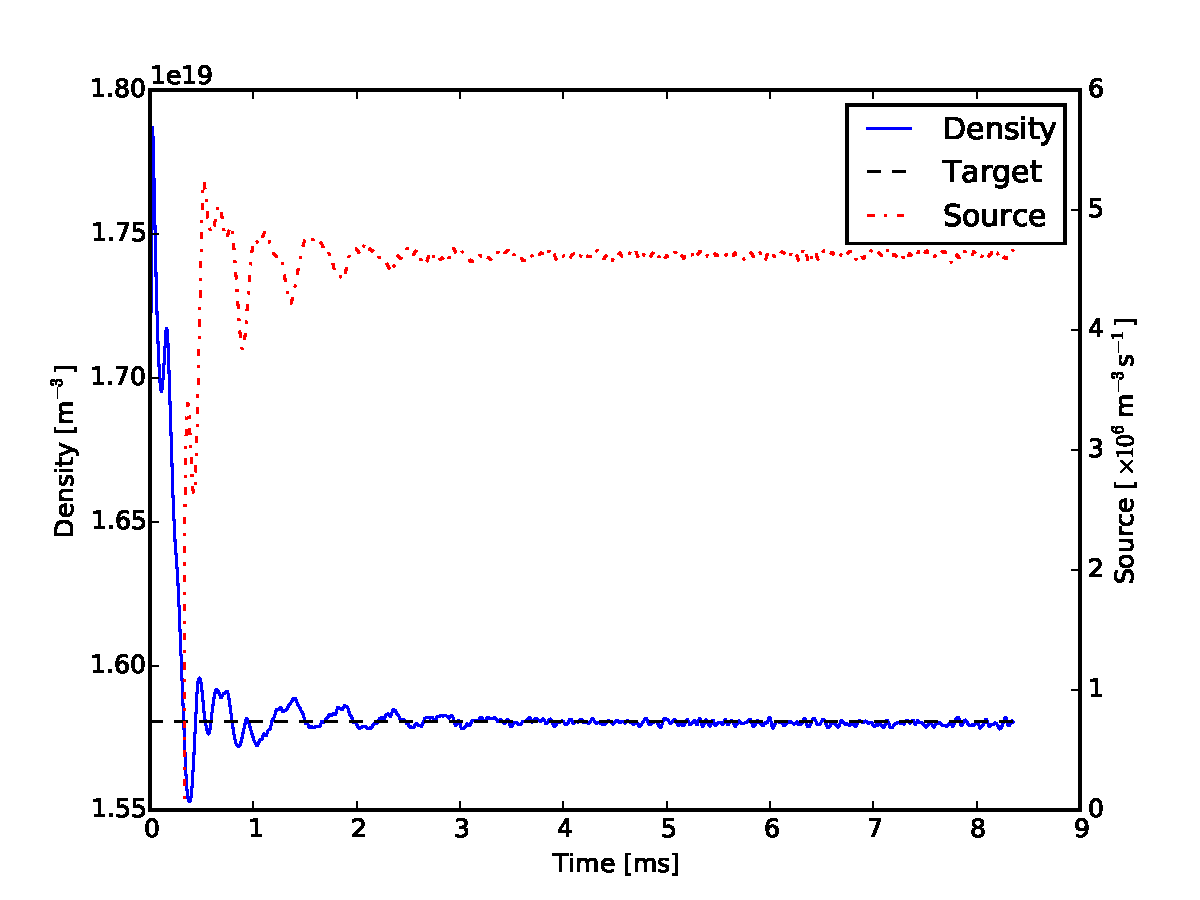
\includegraphics[width=0.7\columnwidth]{figs/DIII-D/density_feedback.pdf}
\caption{An example of density feedback in the \texttt{neutrals-d3d} test case}
\label{fig:density_feedback}
\end{figure}

\subsection{Fixed sources}

Fixed sources are read from the options
\begin{verbatim}
[Ne]
source = ...

[Pe]
source = ...
\end{verbatim}
which are read into the variables $S_n$ and $S_p$ then divided by \texttt{Omega\_ci}.

Terms is then added to the density and pressure equations:
\begin{eqnarray}
  \frac{\partial n}{\partial t} &=& \ldots + \left\{\begin{array}{cc}
  S_n & \mathrm{if} S_n > 0 \\
  n S_n & \mathrm{if} S_n < 0
  \end{array}\right. \\
  \frac{\partial p_e}{\partial t} &=& \ldots + \left\{\begin{array}{cc}
  S_p & \mathrm{if} S_p > 0 \\
  p_e S_p & \mathrm{if} S_p < 0
  \end{array}\right. \\
\end{eqnarray}

The purpose of the switch is so that neither density nor pressure can be forced negative due to a sink term.

\section{Neutral model}
\label{sec:neutrals}

The model used is controlled by the switch

\begin{verbatim}
neutral_model
\end{verbatim}

This can have the following values:

\begin{tabular}{ll}
Value & Meaning \\
\hline
\hline
0 & No neutrals \\
1 & Diffusive model in X-Z \\
2 & Recycling model \\
3 & Fluid model in X-Y \\
4 & Diffusive in X-Z, fluid in Y (UEDGE-like) \\
\hline
\hline
\end{tabular}

\subsection{Diffusive neutral model}

In the simplest neutral model, neutral gas is modelled as a fluid with a density $n_n$ which diffuses with a diffusion coefficient $D_n$:
\begin{equation}
 \frac{\partial n_n}{\partial t} = \nabla\cdot\left(D_n\nabla n_n\right) + S - n_n / \tau_n
\end{equation}
The temperature of the neutrals is assumed to be the same as the ions
$T_n = T_i$.Diffusion of neutrals depends on the neutral gas temperature, and on the collision rate:
\begin{equation}
D_n = v^2_{th,n} / \left(\nu_{cx} + \nu_{nn}\right)
\end{equation}
where $v_{th,n} = \sqrt{eT_n/m_i}$ is the thermal velocity of a neutral atom; $\nu_{cx} = n\sigma_{cx}$ is the charge-exchange
frequency, and $\sigma_{nn} = v_{th,n} n_n a_0$ is the neutral-neutral collision frequency 
where $a_0 \simeq \pi \left(5.29\times 10^{-11}\right)^2$~m$^2$ is the cross-sectional area of a neutral Hydrogen atom. In order to prevent divide-by-zero problems at low densities, which would cause $D$ to become extremely large,
the mean free path of the neutrals is limited to $1$m. 

An additional loss term is required in order to prevent the particle inventory of the simulations becoming unbounded in detached simulations, where recycling no longer removes particles from the system. This represents the
residence time for neutral particles in the divertor region, which in [Togo 2013] was set to around $10^{-4}$s.

\subsection{Recycling model}
This recycling model assumes that the neutral density exponentially falls away from the divertor plate.
\begin{equation}
n_n = n_{n0} e^{-y/\lambda} \label{eqn:exp_neutral_density}
\end{equation}
where $n_{n0}$ is a constant that will need to be calculated and $\lambda$ is the mean-free path of a neutral Deuterium atom.  This mean-free path is a combination of charge exchange and ionization mean free paths, 
\begin{equation}
\lambda = \sqrt{\lambda_{cx}\lambda_{is}} = \frac{v_{th}}{\sqrt{\langle\sigma v\rangle_{cx} \langle\sigma v\rangle_{is} }}
\end{equation}
where $\langle\sigma v\rangle$ is the cross-section rate for the charge-exchange (cx) and ionisation (is) reactions, and $v_{th}$ is the thermal speed, which is determined by assuming the neutral temperature is the Frank-Condon energy (3.5eV).  This approach should allow the simulations to be much faster than including a full neutral fluid model in the next section.\\
\\
The goal of this method is to conserve a fraction, $f_r$, of the particles that hit the divertor, assuming that they are recycled back and re-ionised.
\begin{equation}
\deriv{N_{\text{rec}}}{t} = f_r \deriv{N_{\text{lost}}}{t}  % _{\text{rec}}
\end{equation}
The rate at which particles are lost can be defined as the flux out (at the divertor plate) times the surface area:
\begin{equation}
\deriv{N_{\text{lost}}}{t} = nv_{i\parallel} A 
\end{equation} 
where $A$ is the area on the divertor plate, which is \emph{not} perpendicular to the magnetic field line, so it is important to scale this by the square root of the covariant metric tensor term, $\displaystyle\sqrt{g_{22}}$.  The source term, which is the rate of particle recycling, can be defined using the ionisation cross-section, neutral density, and plasma density.
\begin{equation}
S_n = \deriv{N_{\text{rec}}}{t} = \int n_e n_n \langle \sigma v \rangle_{is} dV
\end{equation}
where $\langle\sigma v\rangle_{is}$ is the ionisation cross-section rate and the integral is over the entire volume of the simulation.  By substituting equation this becomes
\begin{equation}
\deriv{N_{\text{rec}}}{t} = n_{n0} \int n_e e^{-y/\lambda} \langle \sigma v \rangle_{is} dV.
\end{equation}
Now, substituting equations  and into results in an equation for the neutral density constant, $n_{n0}$ that will give the proper recycling rate.
\begin{equation}
n_{n0} = \frac{f_r nv_{i\parallel}A}{\int n \langle\sigma v\rangle_{is} e^{-y/\lambda}dV} 
\end{equation}
The neutral density will evolve such that the recycling rate $f_r$ is maintained along each field line individually.  The flux of particles lost to the divertor on a single field line will be recycled to the same field line.

\subsection{Fluid neutral model}

This model evolves the equations for a neutral fluid, assuming
axisymmetry (constant in Z), for the density $n_n$, velocity $\mathbf{v}_n$
and pressure $p_n$.

\begin{eqnarray}
\frac{\partial n_n}{\partial t} &=& -\nabla\cdot\left(n_n\mathbf{v}_n\right) \nonumber \\
\frac{\partial \mathbf{v}_n}{\partial t} &=& - \mathbf{v}_n\cdot\nabla\mathbf{v}_n -\frac{1}{n_n}\nabla p_n + \frac{1}{n_n}\nabla\cdot\left(\mu \nabla\mathbf{v}\right) + \frac{1}{n_n}\nabla\left[ \left(\frac{1}{3}\mu + \zeta\right)\nabla\cdot\mathbf{v}_n\right] \\
\frac{\partial p_n}{\partial t} &=& -\nabla\cdot\left(p_n\mathbf{v}_n\right) - \left(\gamma - 1\right)p_n\nabla\cdot\mathbf{v}_n + \nabla\cdot\left(\kappa_n \nabla T_n\right) \nonumber
\end{eqnarray}
where the dissipation parameters $\mu$, $\zeta$ and $\kappa$ are constants
set in the \texttt{[neutral]} section of the options:

\begin{center}
\begin{tabular}{ccc}
Variable & Option & Meaning \\
\hline
\hline
$\mu$ & \texttt{viscosity} & Dynamic viscosity \\
$\zeta$ & \texttt{bulk} & Bulk (volume) viscosity \\
$\kappa_n$ & \texttt{conduction} & Thermal conduction \\
\hline
\hline
\end{tabular}
\end{center}


The contravariant components of $\mathbf{v}_n$ are evolved in the same $\left(x,y,z\right)$ field-aligned coordinate system as the plasma. 
To evaluate the nonlinear advection term, whilst avoiding
the use of noisy Christoffel symbols coming from derivatives of basis vectors, these components are transformed into $\left(R,Z,\phi\right)$ cylindrical coordinates, advected, then transformed back. This is done using matrices which are calculated in the initialisation stage by finite differences of the input mesh:

\begin{eqnarray}
  \left(\begin{array}{c}
\nabla R \\
\nabla Z\end{array}\right) &=& \left(\begin{array}{cc}
\frac{\partial R}{\partial x} & \frac{\partial R}{\partial y} \\
\frac{\partial Z}{\partial x} & \frac{\partial Z}{\partial y}\end{array}\right)\left(\begin{array}{c}
\nabla x \\
\nabla y\end{array}\right) \\
&=& \left(\begin{array}{cc}
\texttt{Urx} & \texttt{Ury} \\
\texttt{Uzx} & \texttt{Uzy} \end{array}\right)\left(\begin{array}{c}
\nabla x \\
\nabla y\end{array}\right)
\end{eqnarray}

These components are calculated by finite differences of the
\texttt{Rxy} and \texttt{Zxy} arrays in the input, then adjusted to
match the given values of \texttt{hthe} and \texttt{Bpxy}:
\[
\sqrt{\left(\frac{\partial R}{\partial y}\right)^2 + \left(\frac{\partial R}{\partial y}\right)^2} = h_\theta
\]
\[
\sqrt{\left(\frac{\partial R}{\partial x}\right)^2 + \left(\frac{\partial R}{\partial x}\right)^2} = 1 / \left(R B_\theta\right)
\]
(Note that this second equality only works if $x$ and $y$ are orthogonal).

This matrix is then inverted, to give:
\begin{eqnarray}
  \left(\begin{array}{c}
\nabla x \\
\nabla y\end{array}\right) &=& \left(\begin{array}{cc}
\texttt{Txr} & \texttt{Tyr} \\
\texttt{Txz} & \texttt{Tyz} \end{array}\right)\left(\begin{array}{c}
\nabla R \\
\nabla Z\end{array}\right)
\end{eqnarray}

The components of $\mathbf{v}_n$ are evolved in covariant form:
\begin{equation}
\mathbf{v}_n = v_x \nabla x + v_y \nabla y + v_z \nabla z
\end{equation}
which is then transformed to $v_r$ and $v_Z$:
\begin{eqnarray*}
v_r &=& \mathbf{v}_n \cdot \nabla R = \frac{\partial x}{\partial R} v_x + \frac{\partial y}{\partial R} v_y \\
v_Z &=& \mathbf{v}_n \cdot \nabla Z = \frac{\partial x}{\partial Z} v_x +  \frac{\partial y}{\partial Z} v_y
\end{eqnarray*}
which are implemented as
\begin{verbatim}
Field2D vr = Txr * Vn2D.x + Tyr * Vn2D.y;
Field2D vz = Txz * Vn2D.x + Tyz * Vn2D.y;
\end{verbatim}
These components are then advected as scalars for the $\mathbf{v}_n\cdot\nabla\mathbf{v}_n$ term, and are diffused for the $\nabla\cdot\left(\mu \nabla\mathbf{v}\right)$ dynamic viscosity term. The quantity $\left(\frac{1}{3}\mu + \zeta\right)\nabla\cdot\mathbf{v}_n$ is treated as a pressure (with the same boundary conditions as $p_n$), and calculated in field-aligned coordinates.


At boundaries neutral thermal energy is lost at a rate controlled by the option
\begin{verbatim}
neutral_gamma = 5./4
\end{verbatim}
This sets the flux of power to the wall to:
\[
q = \gamma n_n T_n c_s
\]
Currently this is only done at target boundaries, not radial boundaries.

\subsection{Diffusive fluid model}
\label{sec:uedgeneutrals}

This model (\texttt{neutral\_model = 4}) solves fluid equations along $y$, and uses diffusive transport in X and Z. 
It was adopted from the approach used in UEDGE and this paper [Journal of Nuclear Materials, vol. 313-316, pp. 559-563 (2003)].

\begin{eqnarray*}
  \frac{\partial n_n}{\partial t} &=& -\nabla\cdot\left(n_n\mathbf{b}v_{||n} + n_n\mathbf{v}_{\perp n}\right) + S\\
  \frac{\partial}{\partial t}\left(n_nv_{||n}\right) &=& -\nabla\cdot\left(n_nv_{||n} \mathbf{b}v_{||n} + n_nv_{||n}\mathbf{v}_{\perp n}\right) - \partial_{||}p_n + \nabla_{||}\left(D_{nn}n_n\partial_{||}v_{||n}\right) + F \\
  \frac{\partial p_n}{\partial t} &=& -\nabla\cdot\left(p_n\mathbf{b}v_{||n} + p_n\mathbf{v}_{\perp n}\right) - \frac{2}{3}p_n\nabla\cdot\left(\mathbf{b}v_{||n}\right) + \nabla\cdot\left(D_{nn}n_n\nabla_\perp T_n\right) + \frac{2}{3}Q
\end{eqnarray*}
The parallel momentum is evolved, so that it can be exchanged with the plasma parallel momentum, but the mass is neglected for perpendicular motion. In the perpendicular direction, therefore, the motion is a balance between the friction (primarily with the plasma through charge exchange) and the pressure gradient:
\begin{equation}
  \mathbf{v}_{\perp n} = -D_{nn}\frac{1}{p_n}\nabla_\perp p_n
\end{equation}

At the moment there is no attempt to limit these velocities, which has been found necessary in UEDGE to get physical results in better agreement with kinetic neutral models [Discussion, T.Rognlien].

The perpendicular diffusion terms use a Laplacian operator
which includes y derivatives, \texttt{Div\_Perp\_Lap\_XYZ}

\subsection{Transfer terms}

Plasma fluid and neutral models are coupled through sources and sinks of particles, momentum and energy.
In addition there are external sources:
\begin{itemize}
\item $S_n = $ Source of plasma ions
\item $S_p = $ Source of pressure, related to energy source $S_E = \frac{3}{2}S_p$
\end{itemize}
In the simulations carried out so far, these source functions are both constant between midplane and X-point, and zero
from X-point to target.

There are several transfer channels and sinks for particles, energy and momentum due to rates
of recombination, ionisation and charge exchange:
\begin{eqnarray*}
  \mathcal{R}_{rc} &=& n^2\left<\sigma v\right>_{rc}   \qquad \mbox{\textrm{(Recombination)}} \\
  \mathcal{R}_{iz} &=&  nn_n\left<\sigma v\right>_{iz} \qquad \mbox{\textrm{(Ionisation)}} \\
  \mathcal{R}_{cx} &=& nn_n\left<\sigma v\right>_{cx} \qquad \mbox{\textrm{(Charge exchange)}}
\end{eqnarray*}
where $n$ is the plasma density, and $n_n$ is the neutral gas density. These all have units of m$^{-3}$s$^{-1}$.

\begin{itemize}
\item $S = $ Net recombination i.e neutral source (plasma particle sink). Calculated as Recombination - Ionisation:
\begin{eqnarray*}
  S &=& \mathcal{R}_{rc} - \mathcal{R}_{iz}
\end{eqnarray*}
\item $R = $ Cooling of the plasma due to radiation, and plasma heating due to 3-body recombination at temperatures less than 5.25eV.
  \begin{eqnarray*}
    R &=& \left(1.09 T_e - 13.6\textrm{eV}\right)\mathcal{R}_{rc} \qquad \mbox{\textrm{(Recombination)}}\\
    &+& E_{iz}\mathcal{R}_{iz}  \qquad \mbox{\textrm{(Ionisation)}}
  \end{eqnarray*}
  The factor of 1.09 in the recombination term, together with factor of $3/2$ in $E$ below, is so that recombination becomes a net heat source for the plasma at $13.6 / 2.59 = 5.25$eV. $E_{iz}$ is the average energy required to ionise an atom, including
  energy lost through excitation. Following Togo {\it et al.}, $E_{iz}$ is chosen to be 30eV.
\item $E = $ Transfer of energy to neutrals.
  \begin{eqnarray*}
    E &=& \frac{3}{2} T_e \mathcal{R}_{rc} \qquad \mbox{\textrm{(Recombination)}} \\
    &-& \frac{3}{2} T_n \mathcal{R}_{iz}  \qquad \mbox{\textrm{(Ionisation)}} \\
    &+& \frac{3}{2}\left(T_e - T_n\right)\mathcal{R}_{cx} \qquad \mbox{\textrm{(Charge exchange)**}}
  \end{eqnarray*}
  (**) Note that if the neutral temperature is not evolved, then $T_n = T_e$ is used to calculate
  the diffusion coefficient $D_n$. In that case, $T_n$ is set to zero here, otherwise it would
  cancel and leave no CX energy loss term.
\item $F = $ Friction, a loss of momentum from the ions, due to charge exchange and recombination. 
The momentum of the neutrals is not currently modelled, so instead any momentum lost from the ions 
is assumed to be transmitted to the walls of the machine. 
\begin{eqnarray*}
  F &=& m_iV_{||}\mathcal{R}_{rc} \qquad \mbox{\textrm{(Recombination)}} \\
  &+& m_iV_{||}\mathcal{R}_{cx}  \qquad \mbox{\textrm{(Charge exchange)}}
\end{eqnarray*}
\end{itemize}
Where $\sigma_{cx}$ is the cross-section for charge exchange, $\sigma_{rc}$ is the cross-section for recombination,
and $\sigma_{iz}$ is the cross-section for ionisation. Each of these processes' cross-section depends on the
local density and temperatures, and so changes in time and space as the simulation evolves.

\subsection{Atomic cross sections}

Cross sections are approximated with semi-analytic expressions. 
For the purposes of calculating these cross-sections, any temperatures below 1eV are set to 1eV. 
The charge exchange cross-section is approximated as:
\begin{equation}
  \sigma_{iz} = \left\{\begin{array}{ll}
10^{-14} T^{1/3} & \textrm{if $T \ge 1$eV} \\
10^{-14} & \textrm{if $T < 1$eV} \end{array}\right.
\end{equation}
with units of $[\textrm{m}^3/\textrm{s}]$. Ionisation is calculated as
\begin{equation}
\sigma_{cx} = \left\{\begin{array}{ll}
5.875\times 10^{-12}\cdot T^{-0.5151} \cdot 10^{-2.563/\log_{10}T} & \textrm{if $T \ge 20$eV} \\
10^{-6}\cdot T^{-3.054}\cdot 10^{-15.72\exp\left(-\log_{10}T\right) + 1.603\exp\left(-\log^2_{10}T\right)} & \textrm{if $1$eV $ < T < 20$eV} \\
7.638\times 10^{-21} & \textrm{if $T \le 1$eV}\end{array}\right.
\end{equation}
Recombination rates are calculated using a $9\times 9$ table of coefficients
so is not reproduced here.

\begin{figure}[h]
\centering
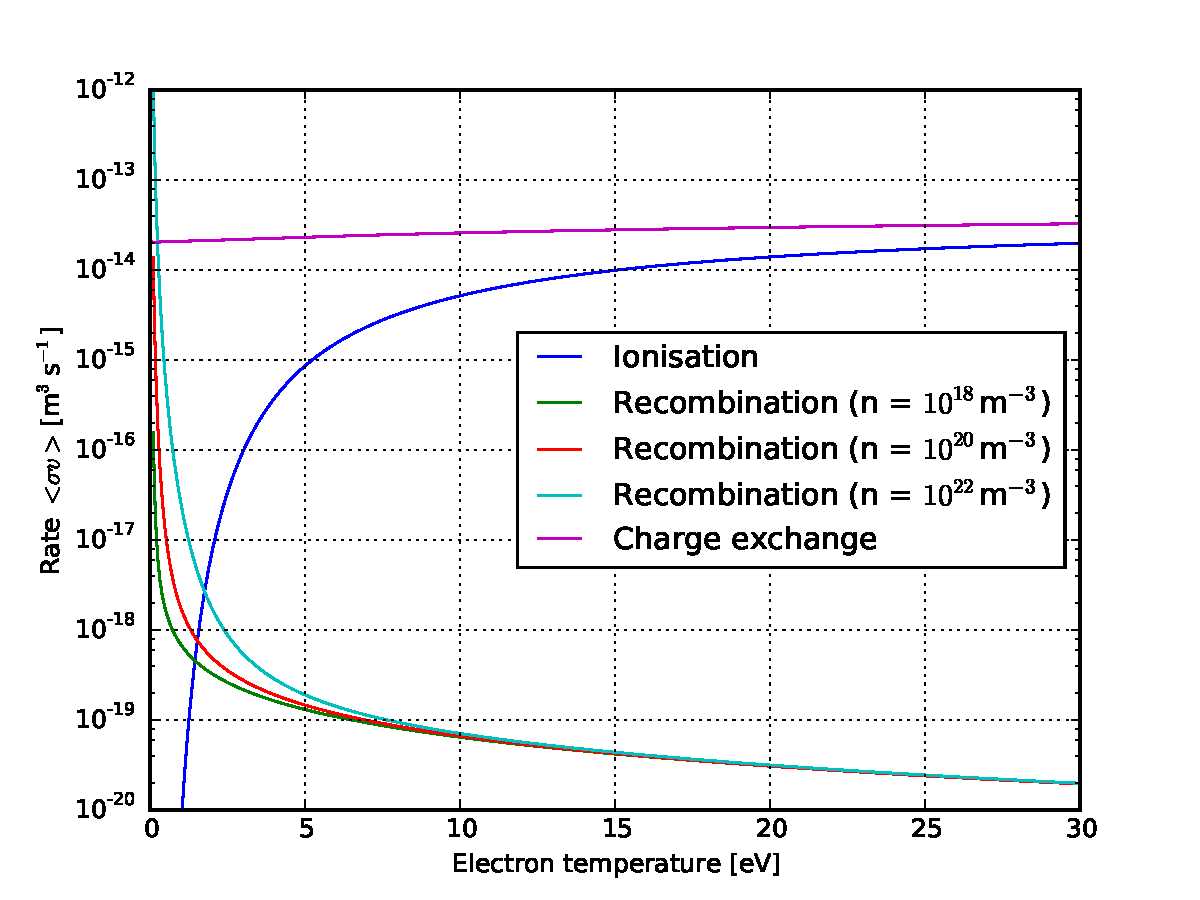
\includegraphics[width=0.7\columnwidth]{figs/hydrogen.pdf}
\caption{Cross-sections [Thanks to H.Willett]}
\label{fig:sigma}
\end{figure}
Plots of these cross-sections are shown in figure~\ref{fig:sigma}. There are a few anomalies with this: charge exchange always has the highest cross-section of any process, and ionisation has a jump at $20$eV. The ionisation and
charge exchange rates do not depend on density, but recombination does so a typical range of values is shown.

\subsection{Impurities}

A fixed carbon fraction can be added by using the setting
\begin{verbatim}
  carbon_fraction = 0.01  # 1% carbon fraction
\end{verbatim}
This only affects the plasma pressure, by adding a radiation loss term. At the moment
the analytic carbon cooling curve from Hutchinson's paper (shown in figure~\ref{fig:carbon}) is used.
\begin{figure}[h]
\centering
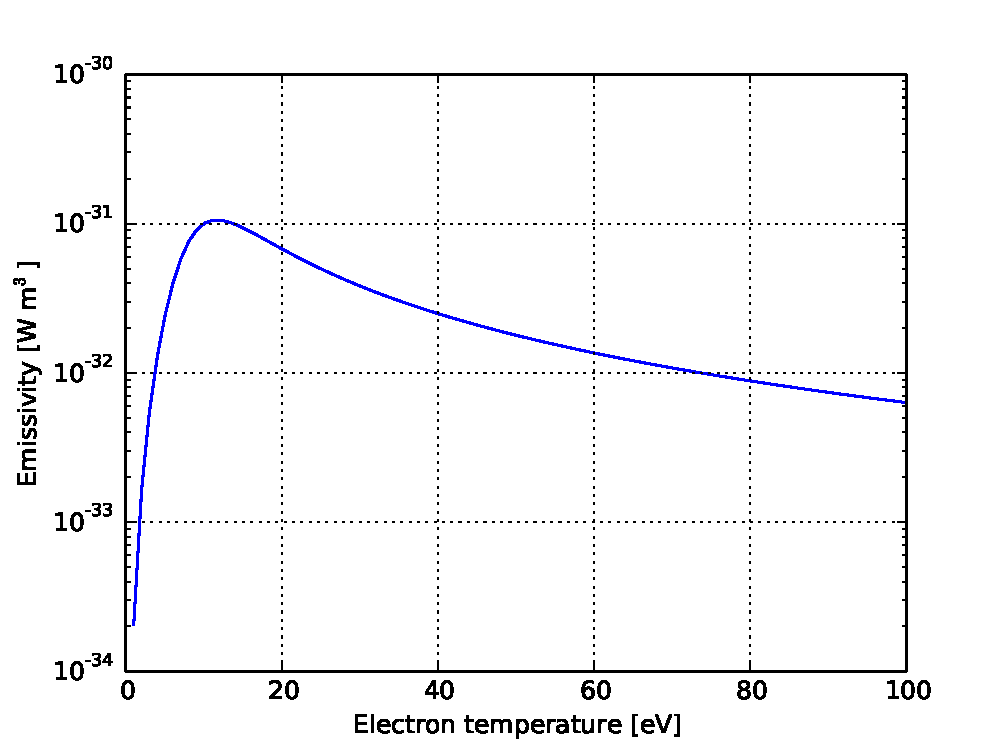
\includegraphics[width=0.7\columnwidth]{figs/carbon_rad.pdf}
\caption{Carbon cooling rate [Hutchinson]}
\label{fig:carbon}
\end{figure}
A negative value indicates that there is no carbon, so the default is -1. 
This is only different from 0.0 in efficiency; if negative then the radiation will not be calculated.

\section{Simulation startup procedure}

Obtaining a steady state can require long simulation times, particularly if the initial conditions are not a good
guess for what the final state looks like. To avoid violent transients and excessive simulation time evolving
a large system of equations from an unphysical starting point, a step-by-step startup procedure can be followed:
\begin{enumerate}
\item Start without any neutrals (\texttt{neutral\_model = 0}), specifying sources of particles near the target plates.
  Run for a timescale of few $\times 10^3 / \Omega_{ci}$, then adjust the sources and run for a bit longer. The idea
  is not to reach equilibrium, but to get past the initial transients when the flow into the sheath begins, which can
  lead to problems for the neutral gas models.
\item Switch on the neutral model with a small recycling fraction (say 10\%)
\item Increase the recycling fraction whilst decreasing the plasma particle source
\item Once the desired recycling fraction is reached, turn off the external particle source,
  and run for as long as needed to get an equilibrium
\item Turn on plasma currents to evolve the electric field
\item Add points in Z...
\end{enumerate}

\section{Boundary conditions}
\label{sec:boundary}

The current through the sheath is described in terms of electron and ion current
\[
j_{sh} = en_{sh}\left(v_{sh,i} - v_{sh,e}\right)
\]
The ion current is just determined by the ion sheath velocity $v_{sh,i}$.
The electron velocity is given by
\begin{equation}
v_{sh,e} = \left\{\begin{array}{ll}
  \sqrt{\frac{eT_e}{m_e}\frac{1}{4\pi}}e^{-\phi/T_e} & \textrm{If $\phi \ge 0$} \\
  \sqrt{\frac{eT_e}{m_e}\frac{1}{4\pi}} & \textrm{If $\phi < 0$}
\end{array}\right.
\end{equation}
If $\phi < 0$ at the sheath, the electron current saturates. This
prevents unphysically large electron flows at the sheath.

\subsection{Heat flux}

The heat flux is more complicated to impose, since it involves both the thermal energy ($P_e$) and parallel momentum ($nV_{||}$) equations.

Terms which could transport energy out of the system at the sheath in the pressure (thermal energy) equation are
\begin{eqnarray}
  \frac{\partial P_e}{\partial t} &=& -\frac{5}{3}\nabla\cdot\left(P_eV_{||e}\right) \\
  && + \frac{2}{3}\nabla\cdot\left(\kappa\partial_{||}T_e\right) \\
  && + 0.71 \frac{2}{3} \nabla\cdot\left(T_ej_{||}\right) \\
  && - 0.71 \frac{2}{3} j_{||} \partial_{||}T_e \qquad \textrm{Thermal force} \\
  && + \frac{2}{3} v_{||e}\partial_{||} P_e
\end{eqnarray}

In the SimCat code these appear as:
\begin{verbatim}
if(parallel_flow)
  ddt(Pe) -= (5./3)*Div_parP_LtoC(Pe,Ve);
if(thermal_conduction)
  ddt(Pe) += (2./3)*Div_Par_Diffusion(kappa_epar, Te);
if(thermal_flux)
  ddt(Pe) += (2./3)*0.71*Div_parP_LtoC(Te,Jpar);
if(thermal_force)
  ddt(Pe) -= (2./3)*0.71*Jpar*Grad_parP(Te);
if(pe_par) {
  ddt(Pe) += (2./3)* Ve * Grad_parP(Pe);
\end{verbatim}

The final term transfers energy between pressure and momentum equations; the second from last (thermal force) term transfers energy to electromagnetic energy. 
If temperature and pressure are set to zero gradient, then these terms are zero at the sheath and so the energy flux is
\begin{equation}
  \Gamma_E = \frac{5}{2}P_eV_{||e} - 0.71T_ej_{||}
\end{equation}

In the momentum equation the parallel fluxes are due to:
\begin{eqnarray}
  \frac{\partial nV_{||}}{\partial t} &=& -\nabla\cdot\left(nV_{||} V_{||}\right) \\
  && - \partial_{||}P_e
\end{eqnarray}

and so the flux of energy from the system in the momentum equation is
\begin{equation}
  \Gamma_E = \frac{1}{2} nV_{||,sh}^2V_{||,sh} = \frac{1}{2}nT_eC_s
\end{equation}
where $V_{||,sh} \ge c_s$ is the velocity at the sheath.

If currents are neglected, the energy flux through the boundary is therefore:
\[
\Gamma_E = 3nT_eC_s
\]
This amount should therefore be subtracted from the heat flux through the boundary
\[
q = \gamma nT_e C_s
\]
where $\gamma = 5.5 \rightarrow 7.8$ is the sheath energy transmission factor (default 6.5 in model currently).

At the midplane (upstream) boundary, no-flow boundaries are implemented:
\begin{eqnarray}
  \partial_{||}n &=& 0 \\
  \partial_{||}p &=& 0 \nonumber \\
  V_{||} &=& 0 \nonumber \\
  \partial_{||}n_n &=& 0 \nonumber
\end{eqnarray}
and hence $\partial_{||}T = 0$ and $\mathbf{q} = 0$.

At the target plate, normal sheath boundary conditions are applied, so velocity at the sheath entrance
is sonic:
\begin{equation}
V_{||}^{sheath} \ge C_s
\end{equation}
If the velocity just in front of the sheath is supersonic, then a zero-gradient boundary condition is used, but if
the flow in front of the sheath is subsonic then the sound speed is used. The flux of ions to the wall is therefore 
\begin{equation}
\Gamma = n^{sheath}V_{||}^{sheath}
\end{equation}
The temperature gradient is set using the sheath energy transmission factor $\gamma_s$ so 
that the total power flux to the target is the sum of kinetic, convection and conduction:
\begin{equation}
\frac{1}{2}m_inV_{||}^3  + \frac{5}{2}pV_{||} - \kappa_{||e}\partial_{||}T = \gamma_s nTC_s
\end{equation}
This equation is then rearranged to calculate the gradient of $T$ at the boundary. 
The temperature gradient is then limited so that temperature always decreases going
towards the wall. Physically this means that the power to the target is allowed to exceed the sheath
transmission factor.

The particle flux at the target depends on the recycling fraction $\eta$. The flux of neutrals from
the target is 
\[
\Gamma_n = -\eta \Gamma
\]
Typically values of $\eta = 0.9$ were used, i.e. 90\% recycling. 

\section{Numerical dissipation}
\label{sec:dissipation}

For numerical stability, and hence correct convergence, numerical schemes
typically require some form of dissipation. This can be done in many different ways,
though care must be taken not to affect the physics. Note that
all numerical dissipation terms include factors of the mesh spacing,
such that they converge to zero as the mesh is refined.

The terms which are available are currently:
\begin{itemize}
\item \texttt{numdiff} : Viscosities in both electron and ion parallel velocity equations.
  \[
  \frac{\partial}{\partial t} \left(VePsi\right) = \ldots + \nabla_{||}\left(10\times\texttt{numdiff}\delta y^2g_{yy}\partial_{||}v_{||e}\right)
  \]
  \[
  \frac{\partial}{\partial t} \left(NVi\right) = \ldots + \nabla_{||}\left(\texttt{numdiff}\delta y^2g_{yy}\partial_{||}v_{||i}\right)
  \]
\item \texttt{ExBdiff} : Perpendicular dissipation on quantities advected by $E\times B$ velocity
  \[
  \frac{\partial}{\partial t} \left(f\right) = \ldots + \texttt{ExBdiff}\times\nabla\cdot\left(\frac{\delta x^2}{g^{xx}} \nabla_\perp f\right)
  \]
  where $f$ is $\left\{Ne, Vort, NVi, Pe\right\}$
\item \texttt{pardiff} : A parallel velocity driven by pressure gradients
  \[
  v_{||} = -\texttt{pardiff}\times \delta y^2g_{yy}\partial_{||}\log p_e
  \]
  Terms in the density, pressure and ion momentum equations appear as:
  \[
  \frac{\partial}{\partial t} \left(f\right) = \ldots + \nabla_{||}\left(f \times \texttt{pardiff}\times \delta y^2g_{yy}\partial_{||}\log p_e\right)
  \]
\end{itemize}

\section{Operators}
\label{sec:operators}

Several operators have been implemented for SimCat, so that


\section{Simulation cases}

\subsection{2D simulations}

To run 2D (drift-plane) simulations, set \texttt{sinks = true}. This 
switches on the following terms:
\begin{eqnarray}
  \deriv{n}{t} &=& \ldots - \frac{\sqrt{T_i}}{2L_{||}}n \\
  \deriv{p_e}{t} &=& \ldots - \frac{2}{3}\kappa_{||e} \frac{T_e}{L_{||}} - T_e \frac{\sqrt{T_i}}{2L_{||}}n
\end{eqnarray}

In addition, closures are applied to the vorticity equation. If \texttt{sheath\_closure = true} then sheath closure
\[
\deriv{\omega}{t} = \ldots + \frac{1}{L_{||}} n\sqrt{T_e}\left[1 - \sqrt{\frac{m_i}{m_e4\pi}}\exp\left(-\phi/T_e\right)\right]
\]


\subsection{Fluid simulations without EM fields}

Evolving the plasma equations without currents or electromagnetic fields reduces the model
to a set of fluid equations for the parallel dynamics and perpendicular diffusion. Coupled
to a neutral gas model, this allows long simulations on transport times. An example
is the \texttt{neutrals-d3d} test case, which uses neutral model 4 and source
feedback to produce the results in figure~\ref{fig:neutrals-d3d}.
\begin{figure}[h]
\centering
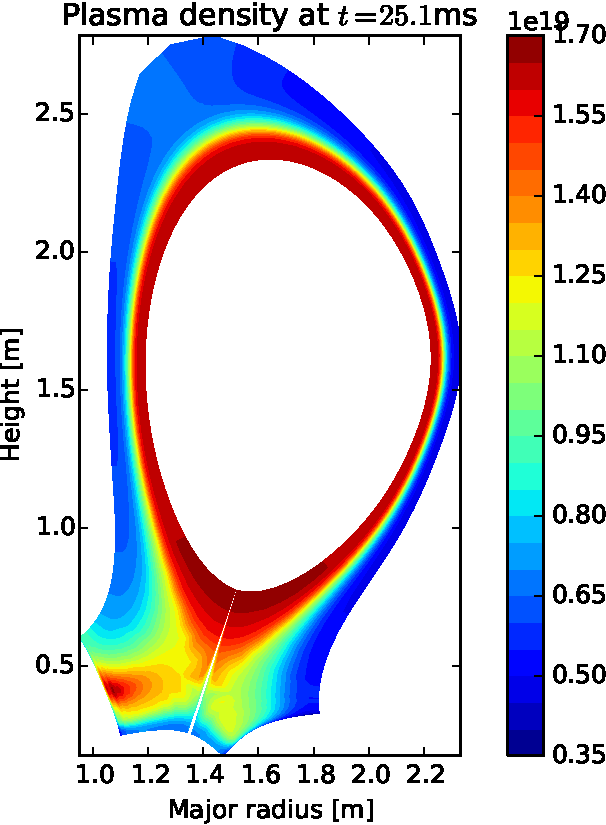
\includegraphics[width=0.24\textwidth]{figs/DIII-D/plasma_density.pdf}
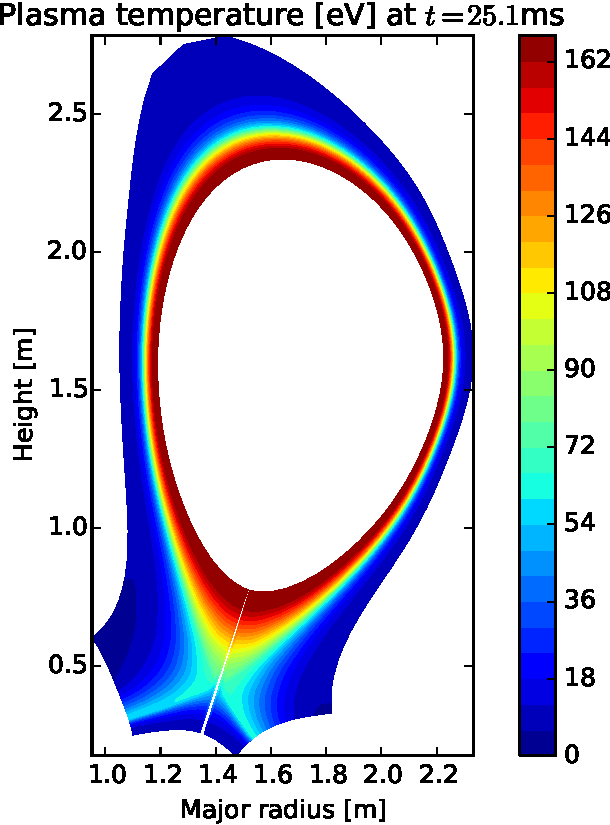
\includegraphics[width=0.24\textwidth]{figs/DIII-D/plasma_temperature.pdf}
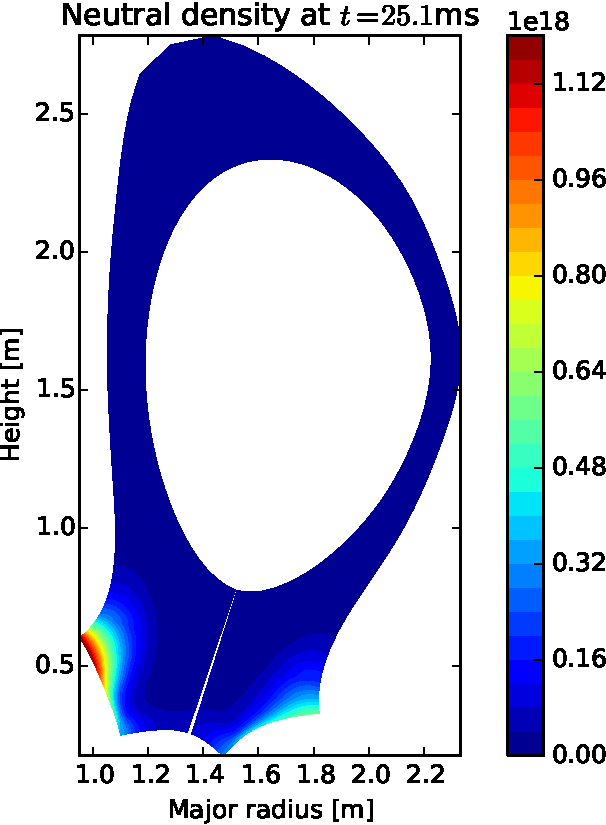
\includegraphics[width=0.24\textwidth]{figs/DIII-D/neutral_density.pdf}
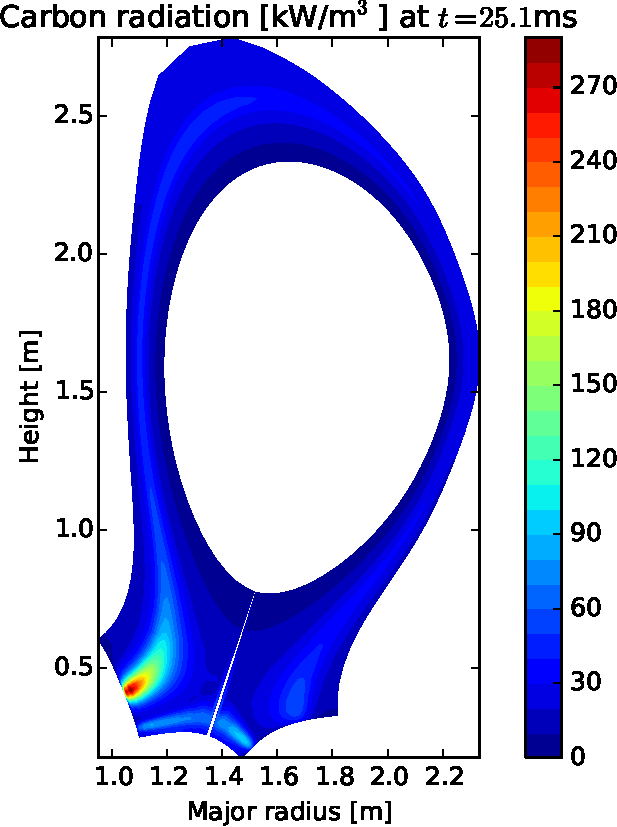
\includegraphics[width=0.24\textwidth]{figs/DIII-D/carbon_radiation.pdf}
\caption{DIII-D fluid transport test case. From left to right are: plasma density, plasma temperature, neutral gas density, and carbon radiation}
\label{fig:neutrals-d3d}
\end{figure}





\subsection{axisym}

Axisymmetric ($n=0$) simulation of Pfirsch-Schluter currents. Starts from a stationary input with
a pressure gradient (and so diamagnetic current) but no parallel current. An $m=1$ electric potential
structure forms initially, oscillates and damps towards a quasi-steady state.

\begin{figure}[h]
\centering
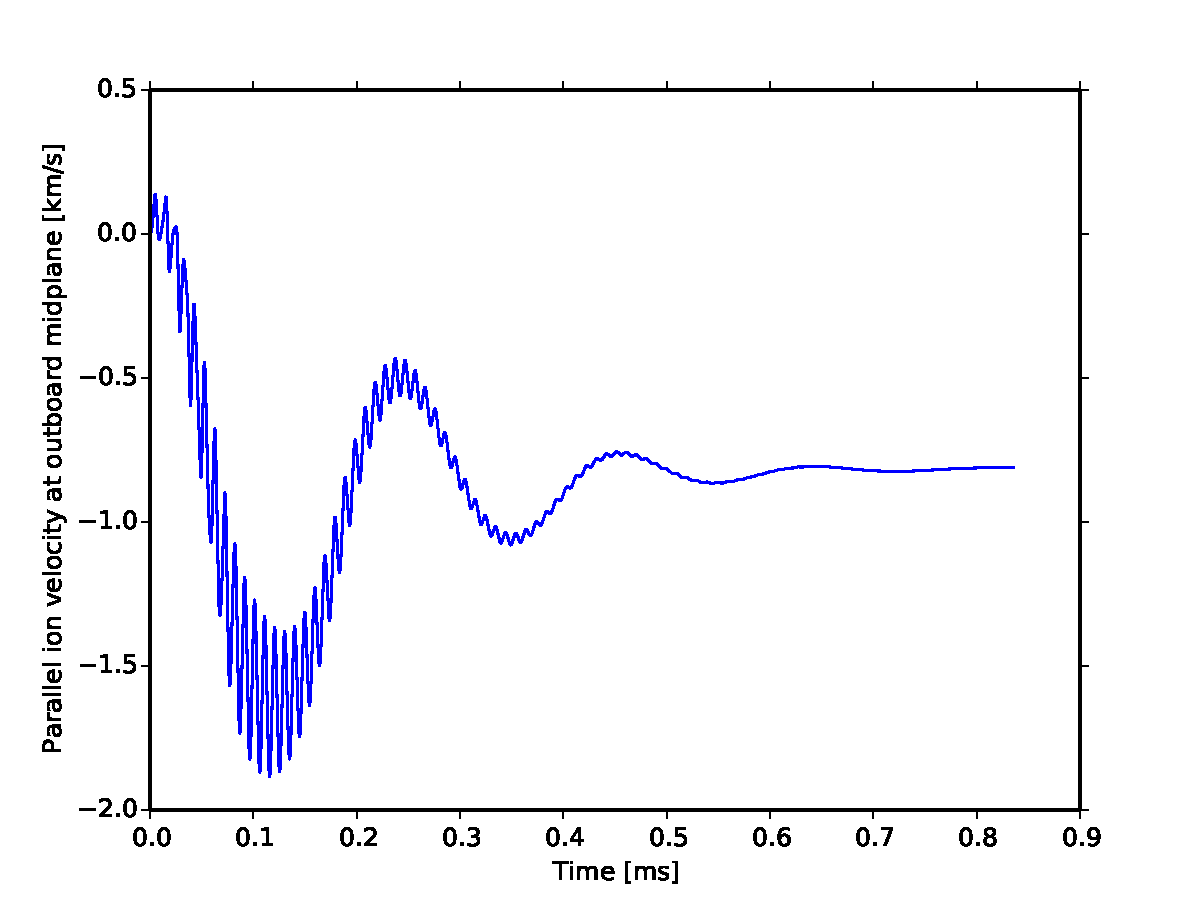
\includegraphics[width=0.32\columnwidth]{figs/axisym-vi-time.pdf}
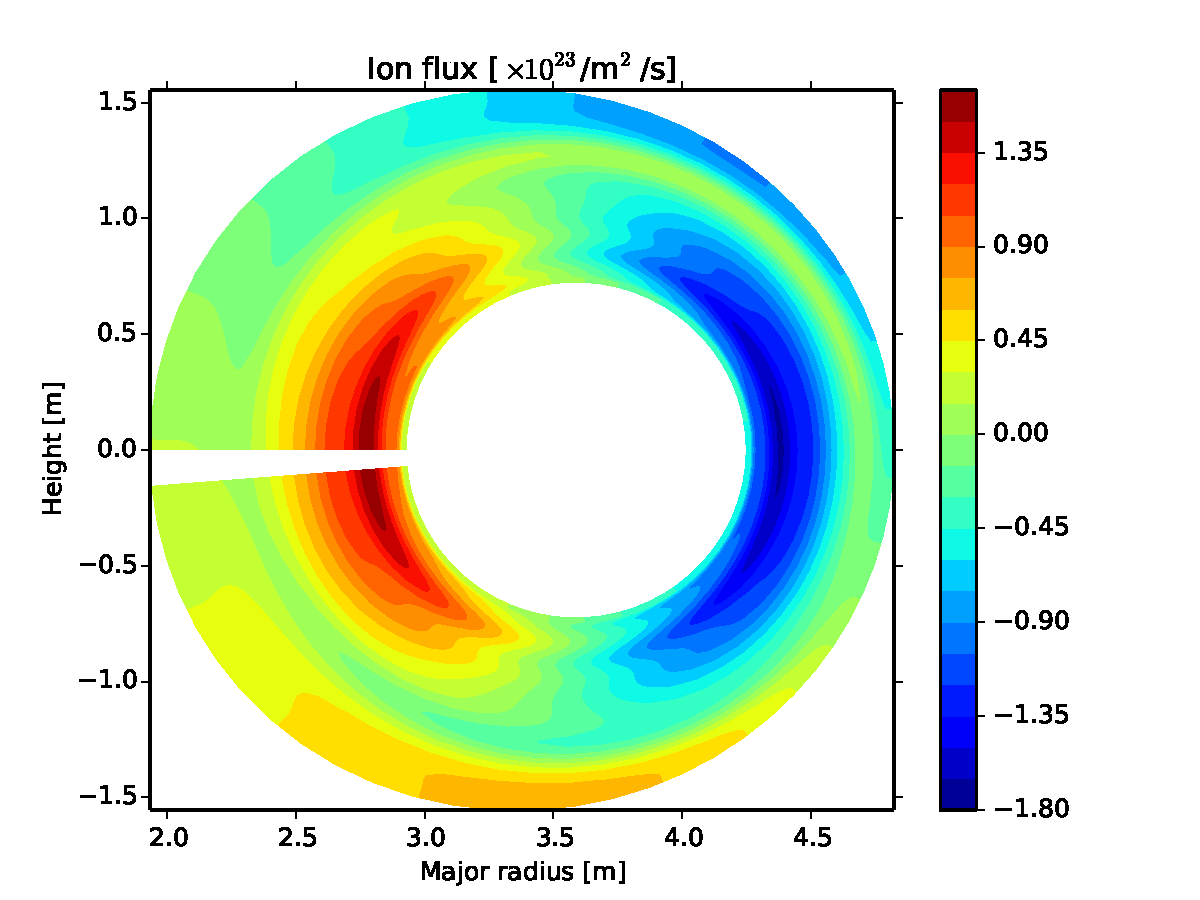
\includegraphics[width=0.32\textwidth]{figs/axisym-ion-flux.pdf}
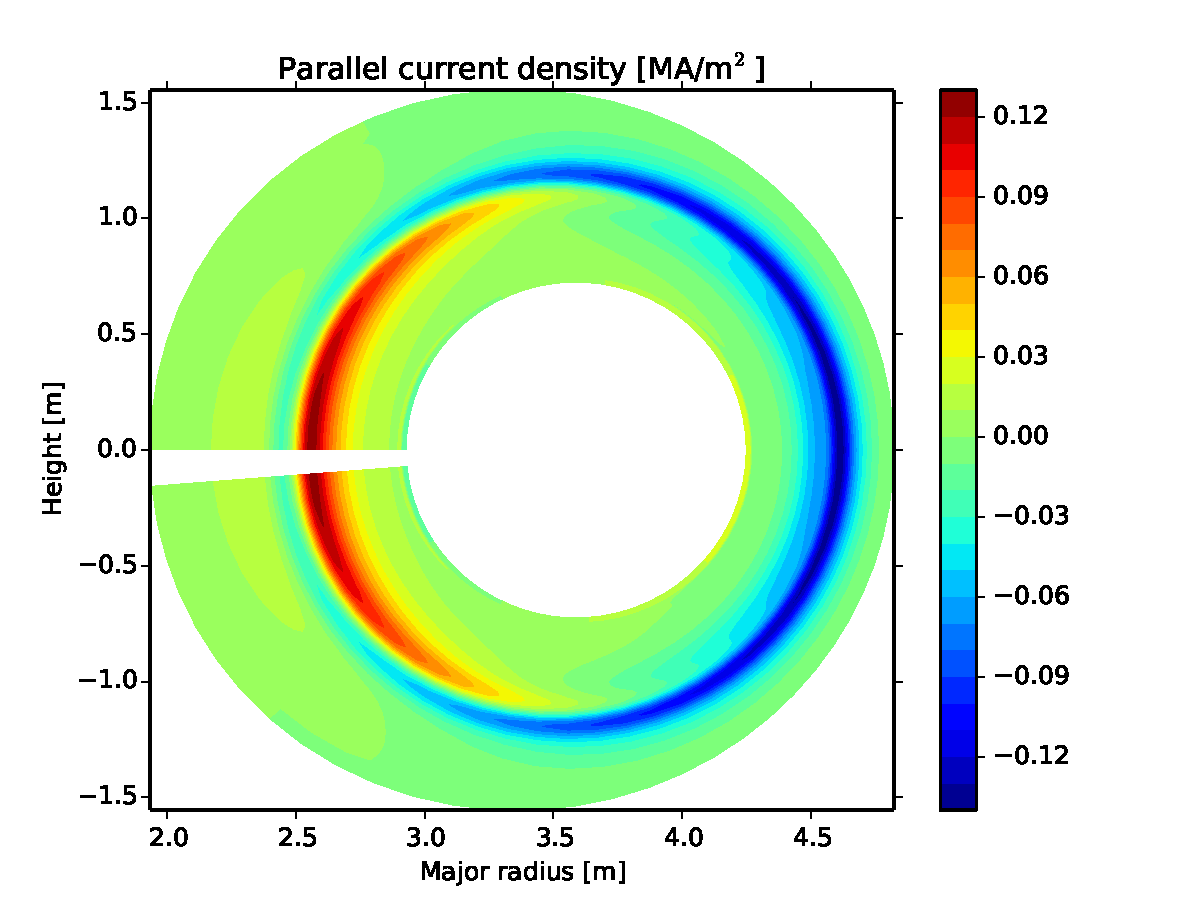
\includegraphics[width=0.32\textwidth]{figs/axisym-jpar.pdf}
\caption{Axisym test case: Transient in parallel ion velocity (left); steady-state ion parallel flux (centre); steady-state parallel current (right)}
\label{fig:axisym}
\end{figure}






\subsection{ISTTOK}

This is a simulation of the circular cross-section, poloidally limited device. The coordinate system
is unusual for BOUT++, in using $z$ as the poloidal angle, and $y$ (parallel) as the toroidal angle.

Starting from an orthogonal toroidal coordinate system consisting of toroidal flux $\psi_t$, poloidal angle $\theta$
and toroidal angle $\zeta$ in which $\mathbf{\hat{e}}_{\psi_t} \times \mathbf{\hat{e}}_\theta = \mathbf{\hat{e}}_\zeta$.
The magnitudes of the vectors are:
\[
\left|\nabla \psi_t\right| = rB_\zeta \qquad \left|\nabla \theta\right| = \frac{1}{r} \qquad \left|\nabla \zeta\right| = \frac{1}{R}
\]
The BOUT++ coordinate system is defined by
\begin{eqnarray}
  x &=& \psi_t \\
  y &=& \zeta \\
  z &=& \frac{1}{q}\zeta - \theta
\end{eqnarray}
(note the sign of $z$ needed to maintain a right-handed coordinate system). For this to be a Clebsch coordinate system
we need the identity:
\begin{equation}
\mathbf{B} = \nabla z \times \nabla x = \frac{1}{J}\mathbf{e}_y
\end{equation}
Substituting we get
\begin{eqnarray}
  \nabla z \times \nabla x &=& \left(\frac{1}{q}\nabla\zeta - \nabla\theta\right)\times\nabla\psi_t \\
  &=& B_\zeta\mathbf{\hat{e}}_\zeta + B_\theta \mathbf{\hat{e}}_\theta = \mathbf{B}
\end{eqnarray}
The Jacobian is given by
\begin{equation}
  J^{-1} = \left(\nabla x \times \nabla y\right) \cdot \nabla z = \frac{B_\zeta}{R}
\end{equation}
The curvature is assumed to be
\begin{equation}
\kappa = -\frac{1}{R}\nabla R
\end{equation}
where from
\[
R = R_0 + r\cos\theta
\]
we get:
\begin{equation}
\nabla R = \cos\theta \nabla r - r \sin\theta = \cos\theta \frac{\nabla \psi_t}{rB_\zeta} - r \sin\theta
\end{equation}
and so
\begin{equation}
  \mathbf{b}\times\mathbf{\kappa} = -\frac{B_\zeta}{BR}\sin\theta \mathbf{\hat{e}}_{\psi_t} - \frac{B_\zeta}{BR}\cos\theta \mathbf{\hat{e}}_\theta + \frac{B_\theta}{BR}\cos\theta \mathbf{\hat{e}}_\zeta
\end{equation}
Taking the dot product with each of the coordinate basis vectors:

\begin{eqnarray}
  \left(\mathbf{b}\times\mathbf{\kappa}\right)\cdot\nabla x &=& -\frac{rB_\zeta^2}{BR}\sin\theta \\
  \left(\mathbf{b}\times\mathbf{\kappa}\right)\cdot\nabla y &=& \frac{B_\theta}{RB^2}\cos\theta \\
  \left(\mathbf{b}\times\mathbf{\kappa}\right)\cdot\nabla z &=& \frac{1}{rR}\left(\frac{B_\zeta}{B} + \frac{B_\theta^2}{B_\zeta B}\right)\cos\theta
\end{eqnarray}

Since we have neglected the poloidal curvature, and are working in large aspect-ratio, the poloidal terms are dropped leaving
only the $x$ and $z$ components:
\begin{equation}
  \left(\mathbf{b}\times\mathbf{\kappa}\right)\cdot\nabla x = -\frac{rB_\zeta^2}{BR}\sin\theta \qquad \left(\mathbf{b}\times\mathbf{\kappa}\right)\cdot\nabla z = \frac{B_\zeta}{BrR}\cos\theta
\end{equation}
If $\theta$ is anticlockwise in the poloidal plane, and $B_\zeta$ is positive, then $\mathbf{b}\times\mathbf{\kappa}$ points
downwards everywhere.


From \url{http://www.cfn.ist.utl.pt/eng/Prj_Tokamak_main_1.html#description}

\begin{tabular}{l c}
R  & 46cm \\
r  &  8.5cm \\
Bt & 0.5T \\
Ip & 7 kA \\
ne (max) & $5e18$m$^-3$ \\
Te (max) & $120$eV \\
q(a) & 5 \\
\end{tabular}

To create the input grid:

\begin{verbatim}
>>> import circle
>>> circle.generate(68,16,512, R=0.46, 
                    r=0.085, dr=0.02, 
                    Bt=0.5, q=5.0, 
                    ixseps=20, 
                    file="isttok.nc")
\end{verbatim}


\end{document}
